%%%%%%%%%%%%%%%%%%%%%%%%%%%%%%%%%%%%%%%%%12pt: grandezza carattere
                                        %a4paper: formato a4
                                        %openright: apre i capitoli a destra
                                        %twoside: serve per fare un
                                        %   documento fronteretro
                                        %report: stile tesi (oppure book)
\documentclass[12pt,a4paper,openright,twoside]{report}
%
%%%%%%%%%%%%%%%%%%%%%%%%%%%%%%%%%%%%%%%%%libreria per scrivere in italiano
\usepackage[italian]{babel}
%
%%%%%%%%%%%%%%%%%%%%%%%%%%%%%%%%%%%%%%%%%libreria per accettare i caratteri
                                        %   digitati da tastiera come è à
                                        %   si può usare anche
                                        %   \usepackage[T1]{fontenc}
                                        %   però con questa libreria
                                        %   il tempo di compilazione
                                        %   aumenta
\usepackage[utf8]{inputenc}
%
%%%%%%%%%%%%%%%%%%%%%%%%%%%%%%%%%%%%%%%%%libreria per impostare il documento
\usepackage{fancyhdr}
%
%%%%%%%%%%%%%%%%%%%%%%%%%%%%%%%%%%%%%%%%%libreria per avere l'indentazione
%%%%%%%%%%%%%%%%%%%%%%%%%%%%%%%%%%%%%%%%%   all'inizio dei capitoli, ...
\usepackage{indentfirst}
%
%%%%%%%%%libreria per mostrare le etichette
%\usepackage{showkeys}
%
%%%%%%%%%%%%%%%%%%%%%%%%%%%%%%%%%%%%%%%%%libreria per inserire grafici
\usepackage{float}

\usepackage{graphicx}
\usepackage{color, colortbl}

%
%%%%%%%%%%%%%%%%%%%%%%%%%%%%%%%%%%%%%%%%%libreria per utilizzare font
                                        %   particolari ad esempio
                                        %   \textsc{}
\usepackage{newlfont}
%
%%%%%%%%%%%%%%%%%%%%%%%%%%%%%%%%%%%%%%%%%librerie matematiche
\usepackage{amssymb}
\usepackage{amsmath}
\usepackage{latexsym}
\usepackage{amsthm}
\usepackage{cite}
\usepackage{listings}
\usepackage{hyperref} 
\usepackage[square,numbers,sort]{natbib} 
\usepackage{xcolor}
\usepackage{url}
%\bibliographystyle{unsrt}
%\bibliographystyle{unsrtnat}

\lstset{
	frame=single,
	breaklines=true
}


%
\oddsidemargin=30pt \evensidemargin=20pt%impostano i margini
\hyphenation{sil-la-ba-zio-ne pa-ren-te-si}%serve per la sillabazione: tra parentesi 
					   %vanno inserite come nell'esempio le parole 
%					   %che latex non riesce a tagliare nel modo giusto andando a capo.

%
%%%%%%%%%%%%%%%%%%%%%%%%%%%%%%%%%%%%%%%%%comandi per l'impostazione
                                        %   della pagina, vedi il manuale
                                        %   della libreria fancyhdr
                                        %   per ulteriori delucidazioni
\pagestyle{fancy}\addtolength{\headwidth}{20pt}
\renewcommand{\chaptermark}[1]{\markboth{\thechapter.\ #1}{}}
\renewcommand{\sectionmark}[1]{\markright{\thesection \ #1}{}}
\rhead[\fancyplain{}{\bfseries\leftmark}]{\fancyplain{}{\bfseries\thepage}}
\cfoot{}
%%%%%%%%%%%%%%%%%%%%%%%%%%%%%%%%%%%%%%%%%
\linespread{1.3}                        %comando per impostare l'interlinea
%%%%%%%%%%%%%%%%%%%%%%%%%%%%%%%%%%%%%%%%%definisce nuovi comandi
%

%%%%%%%%%%%%%%%%%%%%%%%%%%%%%%%%%%%%%%
% Comandi Custom %
%%%%%%%%%%%%%%%%%%%%%%%%%%%%%%%%%%%%%%
\newcommand{\xstudent}{Nome dello studente}
\newcommand{\xsupervisor}{Nome del relatore}



%%%%%%%%%%%%%%%%%%%%%%%%%%%%%%%%%%%%%%
% Fine Preambolo %
% Inizio documento%
%%%%%%%%%%%%%%%%%%%%%%%%%%%%%%%%%%%%%%


\begin{document}

	%%%%%%%%%%%%%%%%%%%%%%%%%%%%%%%%%%%%%%%%
	% Scelta delle dimensioni della pagina %
	%%%%%%%%%%%%%%%%%%%%%%%%%%%%%%%%%%%%%%%%

	%\setlength{\textwidth}{13.5cm}
	%\setlength{\textheight}{19cm}
	%\setlength{\footskip}{3cm}
	
	%%%%%%%%%%%%%%%%%%%%%%%%%
	% inizio prefazione
	%
	% pagina del titolo, indice, sommario
	%%%%%%%%%%%%%%%%%%%%%%%%%
	
	
%\textwidth=450pt
\oddsidemargin=25pt

\begin{titlepage}
\begin{center}
{{\Large{\textsc{Alma Mater Studiorum}}}\\
{\Large{\textsc{Universit\`a di Bologna}}} \\
{\textsc{Campus di Cesena}} \rule[0.1cm]{14cm}{0.1mm}
		\rule[0.5cm]{14cm}{0.6mm}
DIPARTIMENTO DI INFORMATICA – SCIENZA E INGEGNERIA
Corso di Laurea Triennale in Ingegneria e Scienze Informatiche }
\end{center}
\vspace{15mm}
\begin{center}
{\LARGE{\bf Data Visualization e Sonification per aumentare la consapevolezza sull’inquinamento attraverso un'applicazione web interattiva}}\\
\end{center}
\vspace{15mm}
\begin{center}
 {\large{ Elaborato in:\\
Programmazione di Sistemi Mobile\\}}   
\end{center}
\vspace{20mm}
\par
\noindent


\begin{minipage}[t]{0.47\textwidth}
{\large{\bf Relatore:\\
\xsupervisor}}
\end{minipage}


\hfill
\begin{minipage}[t]{0.47\textwidth}\raggedleft
{\large{\bf Presentata da:\\
\xstudent}}
\end{minipage}

\vspace{-8mm}

\begin{minipage}[t]{0.47\textwidth}
{\large{\bf Correlatore:\\
\xcosupervisor}}
\end{minipage}



\vspace{20mm}

\begin{center}
{\large{\bf Sessione II\\%inserire il numero della sessione in cui ci si laurea
Anno Accademico 2021-2022}}%inserire l'anno accademico a cui si è iscritti
\end{center}
\end{titlepage}

	\clearpage{\pagestyle{empty}\cleardoublepage}
\begin{titlepage}                       %crea un ambiente libero da vincoli
                                        %   di margini e grandezza caratteri:
                                        %   si pu\`o modificare quello che si
                                        %   vuole, tanto fuori da questo
                                        %   ambiente tutto viene ristabilito
%
\thispagestyle{empty}                   %elimina il numero della pagina
\topmargin=6.5cm                        %imposta il margina superiore a 6.5cm
\raggedleft                             %incolonna la scrittura a destra
\large                                  %aumenta la grandezza del carattere
                                        %   a 14pt
\em                                     %emfatizza (corsivo) il carattere
%Questa \`e la \textsc{Dedica}:\\
%ognuno pu\`o scrivere quello che vuole, \\
%anche nulla \ldots                      %\ldots lascia tre puntini
\newpage                                %va in una pagina nuova

%
%%%%%%%%%%%%%%%%%%%%%%%%%%%%%%%%%%%%%%%%
\clearpage{\pagestyle{empty}\cleardoublepage}%non numera l'ultima pagina sinistra
\end{titlepage}
    
    %
%%%%%%%%%%%%%%%%%%%%%%%%%%%%%%%%%%%%%%%%
\pagenumbering{roman}                   %serve per mettere i numeri romani
\chapter*{Introduzione}                 %crea l'introduzione (un capitolo
                                        %   non numerato)
%%%%%%%%%%%%%%%%%%%%%%%%%%%%%%%%%%%%%%%%%imposta l'intestazione di pagina
\rhead[\fancyplain{}{\bfseries
INTRODUZIONE}]{\fancyplain{}{\bfseries\thepage}}
\lhead[\fancyplain{}{\bfseries\thepage}]{\fancyplain{}{\bfseries
INTRODUZIONE}}
%%%%%%%%%%%%%%%%%%%%%%%%%%%%%%%%%%%%%%%%%aggiunge la voce Introduzione
                                        %   nell'indice
\addcontentsline{toc}{chapter}{Introduzione}
Questo volume di tesi descrive la progettazione e la realizzazione di un sistema volto ad aumentare la consapevolezza sull'inquinamento atmosferico tramite la sonificazione dei dati sulla qualità dell'aria.
\\\\
La sonificazione è il processo con il quale un dato viene trasformato in un elemento sonoro, aumentandone così la capacità di comunicazione e il coinvolgimento tramite lo stimolo dell'udito.
\\\\
Siccome questo sistema dovrà essere utilizzabile da un pubblico non specializzato, verranno forniti alcuni concetti di base riguardanti l'inquinamento e le metriche utilizzate per la misurazione di questo.
Saranno inoltre elencati i rischi per la salute che il peggioramento della qualità dell'aria comporta, e le principali tipologie di rappresentazione grafica dei dati ambienetali.
\\\\
All'interno di questo testo saranno integrati concetti di produzione sonora e audio digitale, al fine di fornire una panoramica completa sul funzionamento del sistema sonificativo.
Per comprendere il collegamento tra un dato e la sua rappresentazione sonora, saranno discusse le metodogie sonificative solitamente utilizzate, comprese di esempi pratici.

\newpage

\subsubsection{Suddivisione dei contenuti}
Il volume di tesi è composto da tre capitoli principali, ognuno dei quali diviso in più sezioni.
La spartizione dei contenuti è stata fatta in modo da raggruppare gli argomenti seguendo la logica delle fasi di sviluppo del progetto.

\subsubsection{Primo Capitolo}
Il primo capitolo è dedicato ad introdurre il lettore al contesto in cui il progetto si inserisce, e alle motivazioni che hanno portato alla sua realizzazione.
Particolare attenzione è riservata a descrivere il problema dell'inquinamento atmosferico, le sue conseguenze e le tecniche tramite le quali questo viene rappresentato.
Utilizzando un linguaggio non troppo tecnico sarà presentato il concetto di Sonificazione: l'argomento principale del progetto, per poi spiegarne le caratteristiche, le possibili applicazioni, le strategie di realizzazione e alcuni esempi reperibili in rete.
Verranno inoltre introdotte alcune nozioni sulla produzione audio digitale, che verranno approfondite nei capitoli successivi.

\subsubsection{Secondo Capitolo}
Il secondo capitolo è dedicato alla descrizione delle scelte tecniche effettuate per la realizzazione del progetto.
In seguito all'elenco dei requisiti, verranno mostrate alcune schermate relative all'interfaccia utente realizzate in fase di progettazione grafica, e verranno descritte le tecnologie utilizzate per la realizzazione del sistema, giustificandone le scelte.
Il capitolo presta particolare attenzione a distinguere le tecnologie inarenti alla parte web rispetto a quelle utilizzate per la generazione dell'audio;
al termine di questo, sarà possibile avere una panoramica completa dell'architettura del sistema.

\subsubsection{Terzo Capitolo}
Il terzo capitolo descrive in dettaglio le scelete implementative prese durante lo sviluppo del sistema.
Verranno descritte le funzionalità in maniera approfondita: gli argomenti trattati principalmente in questa sottosezione riguardano la realizzazione e la struttura della parte di front-end, e la generazione dell'audio da un punto di vista sia tecnico che musicale.
Infine, verrà discussa la fase di test effettuata a seguito del completamento del progetto: verrà introdotta la metrica adottata per misurare la qualità del sistema, verranno mostrati i risultati ottenuti saranno elencati i problemi riscontrati durante questa fase.



%%%%%%%%%%%%%%%%%%%%%%%%%%%%%%%%%%%%%%%%%non numera l'ultima pagina sinistra
\clearpage{\pagestyle{empty}\cleardoublepage}


\tableofcontents                        %crea l'indice
%%%%%%%%%%%%%%%%%%%%%%%%%%%%%%%%%%%%%%%%%imposta l'intestazione di pagina
\rhead[\fancyplain{}{\bfseries\leftmark}]{\fancyplain{}{\bfseries\thepage}}
\lhead[\fancyplain{}{\bfseries\thepage}]{\fancyplain{}{\bfseries
INDICE}}
%%%%%%%%%%%%%%%%%%%%%%%%%%%%%%%%%%%%%%%%%non numera l'ultima pagina sinistra
\clearpage{\pagestyle{empty}\cleardoublepage}
\listoffigures                          %crea l'elenco delle figure
%%%%%%%%%%%%%%%%%%%%%%%%%%%%%%%%%%%%%%%%%non numera l'ultima pagina sinistra
\clearpage{\pagestyle{empty}\cleardoublepage}
\listoftables                           %crea l'elenco delle tabelle
%%%%%%%%%%%%%%%%%%%%%%%%%%%%%%%%%%%%%%%%%non numera l'ultima pagina sinistra
    
    

	
	%%%%%%%%%%%%%%%%%%%%%%%%%
	% inizio corpo del documento
	%
	% sequenze delle varie sezioni
	% è consigliato mantenere una struttura logica ben definita per separare le sezioni
	% si consiglia di reificare tale struttura fisicamente sul file system
	%%%%%%%%%%%%%%%%%%%%%%%%%
	

	
	% inclusione delle sezioni
	\clearpage{\pagestyle{empty}\cleardoublepage}
\chapter{Background e Contesto}                %crea il capitolo
%%%%%%%%%%%%%%%%%%%%%%%%%%%%%%%%%%%%%%%%%imposta l'intestazione di pagina
\lhead[\fancyplain{}{\bfseries\thepage}]{\fancyplain{}{\bfseries\rightmark}}
\pagenumbering{arabic}                  %mette i numeri arabi

In questo primo capitolo verrà discussa la problematica dell'inquinamento atmosferico.
Saranno elencate le sue cause ed i suoi effetti, e si discuterà sulle modalità tramite le quali viene diffusa la consapevolezza sull'argomento.
Questo capitolo introduttivo si occuperà di fornire il contesto in cui si inserisce il progetto di tesi, prestando particolarmente attenzione all'utilizzo di varie metodologie di rappresentazione dei dati; soffermandosi, in particolare, sui pregi e difetti, proponendo inoltre delle alternative non del tutto convenzionali.

\section{L'inquinamento dell'aria}
Con inquinamento atmosferico, si intendono tutte le alterazioni alla normale composizione chimica, fisica e biologica dell’atmosfera; o più semplicemente dell’aria che respiriamo.
Possiamo dividere le principali cause del peggioramento dell’aria in due categorie: naturali e antropiche.
\\
Le cause naturali dell'inquinamento riguardano principalmente eventi climatici ed ambientali, come ad esempio le eruzioni vulcaniche e le piogge acide.
Questi fenomeni esistono dapprima dell'uomo e non possono essere evitati, nonostante questo; gli inquinanti naturali non rappresentano una minaccia particolarmente seria per la salute umana.
\\
L'inquinamento antropico è invece dovuto alle azioni dell'uomo. Le principali cause di questo sono l’uso di combustibili fossili come il carbone, il petrolio e il gas naturale.
In seguito alla combustione, queste risorse rilasciano sostanze nocive, come ad esempio il monossido di carbonio, la CO\textsubscript{2} e i metalli pesanti.
Fortunatamente, le politiche di tutela dell'ambiente sono sempre più attente a questo problema;
non sono poche neanche le campagne di sesnibilizzazione il cui fine è quello di istruire la popolazione sull'argomento. Questi eventi sono organizzati da enti riconosciuti a livello internazionale e nazionale, come ad esempio l'associazione ambientalista Legambiente: l'associazione dei cittadini per la difesa dell'ambiente ~\cite{la_mincrometrologia}.
\\
\subsubsection{Relazione tra inquinamento e territorio}
Possiamo definire l'inquinamento antropico come una causa della civilizzazione e dell'industrializzazione: il peggioramento della qualità dell'aria è infatti strettamente legato all'urbanizzazione, caratterizzata dall'aumento della popolazione e dei loro bisogni di trasporto, di energia e di beni di consumo.
La relazione tra uomo e inquinamento è molto complessa ed osservabile sotto vari aspetti di cause ed effetto.
Il modo in cui la popolazione si distribuisce nel globo ha un forte impatto sull'ambiente.
Già nel 1999, circa metà della popolazione mondiale (47\%) viveva in aree urbane, a causa della migrazione verso le grandi città.
Questo ha portato, specialmente nelle regioni meno sviluppate, ad un inevitabile surclassamento dell'urbanizzazione rispetto allo svilupo di tecnologie sostenibili e di politiche di tutela dell'ambiente ~\cite{population_and_enviroment}.
\\
Altri fattori che influenzano il preggioramento dell'aria non sono direttamente legati alla popolazione, ma alle caratteristiche naturali del territorio.
La presenza di polveri sottili nell'atmosfera è uno degli aspetti cruciali che influenzano la qualità dell'aria.
Seppure presenti anche in natura, nelle rocce e nelle sabbie, le polveri sottili più nocive sono di causa antropica, e si concentrano nelle metropoli.
Un fenomeno da non sottovalutare è quello del rimescolamento: le particelle inquinanti possono essere trasportate da un luogo all'altro seguendo le correnti di vento, mescolandosi con l'aria pulita.
Il rimescolamento non è però sempre un fenomeno negativo, in quanto può “omogeneizzare”, e quindi mitigare, il livello di inquinamento in un'area molto vasta, riducendo la concentrazione di inquinanti in possibili centri abitati ~\cite{la_mincrometrologia}.

\subsection{Riferimenti legislativi}
In Italia, il principale decreto legislativo che tratta la tematica di inquinamento dell'aria è il 155/2010 “Attenuazione della direttiva 2008/50/UE relativa alla qualità dell'aria ambiente e per un'aria pulita in Europa”.
Le normative emanate in questo decreto si pongono come obbiettivo quello di ridurre l'inquinamento atmosferico, attraverso l'adozione di misure di prevenzione e di controllo.
Il provvedimento individua per ogni Regione gli enti al quale delegare l'utilizzo di strumenti utili alla misuara dell'inquinamento e l'attuazione di piani di prevenzione e risanazione dell'aria.
Il punto principale del decreto è quello di stabilire quali sono le sostanze inquinanti e quali sono i loro livelli massimi tollerabili, al fine di tutelare la salute umana, in particolare quella dei soggetti più deboli ~\cite{arpa_veneto}.
\begin{figure}
  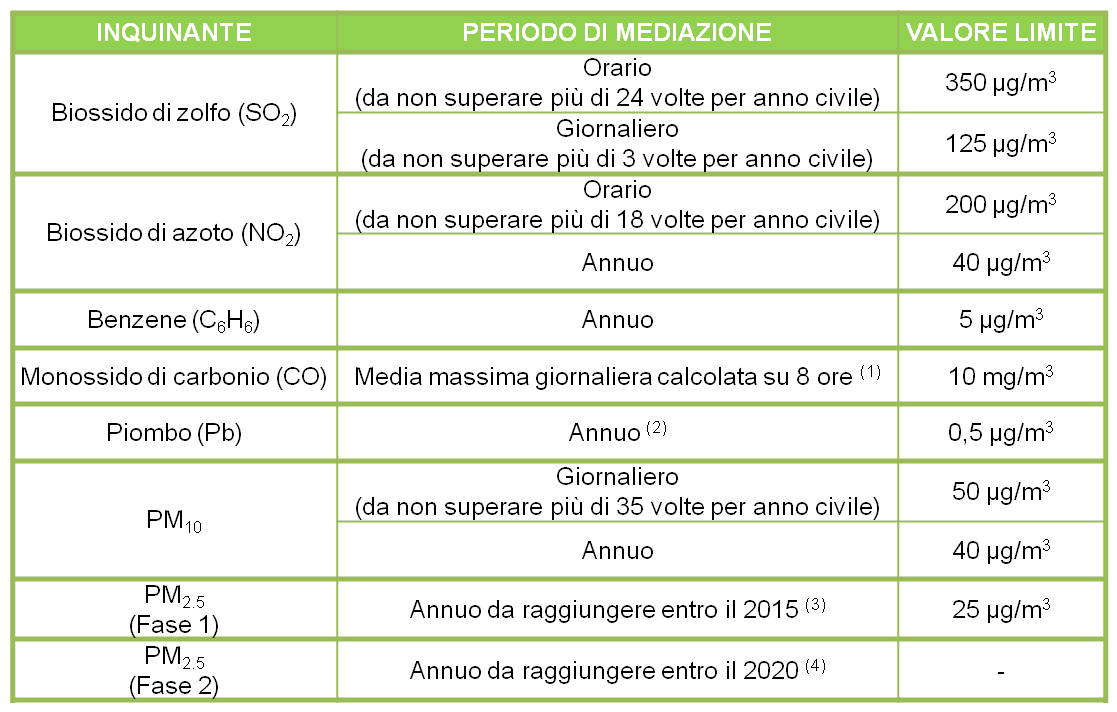
\includegraphics[width=\linewidth]{img/livelli.png}
  \caption{Concentrazione massima tollerata per agente inquinante secondo il decreto 155/2010}
  \label{fig:livelli}
\end{figure}


\subsection{Misurare l'inquinamento}
Per conoscere il livello di qualità dell’aria in una determinata località, è necessario rilevare la concentrazione di ogni elemento nocivo. 
L'ente principale che si occupa di monitorare l'inquinamento atmosferico è la WHO: World Health organization.
\\
La misurazione effettiva dell'inquinamento è delegata alle amministrazioni locali, che si occupano di installare i sensori necessari per rilevare la concentrazione di ogni sostanza.
Negli Stati Uniti, L'EPA è il leader sulla ricerca e sullo sviluppo di strumenti e tecnologie per misurare l'inquinamento atmosferico.
Nell'Unione Europea, invece, questo compito è affidato all' EEA: European Environment Agency.
\\
Ciascuna di queste oraganizzazioni si occupa inoltre di effettuare piani di prevenzione e precauzione per ridurre l'inquinamento all'origine, rivolgendosi alle imprese più impattanti sull'ambiente con la formula “polluter pays”, che vuol dire che chi inquina paga \cite{polluter_pays}.
\\ 
Per semplificare la rappresentazione della condizione dell’aria, l’EPA ha introdotto l’AQI (air quality index): una misurazione semplice e generalizzata.
Ulteriori indici che verranno discussi in questa tesi sono il PM2.5 e il PM10, le cui metodologie di rilevazione sono standardizzate e normate dalla WHO.
Questi valori sono calcolati in base alla concentrazione di particolato aereodisperso di grandezza inferiore a 2.5 e 10 micrometri per metro cubo, rispettivamente.
L'accumulo di queste polveri sottili nell'aria è ciò che viene comunemente definito come smog.
\\
Le particelle sottili PM2.5 sono particolarmente dannose per la salute umana, in quanto possono penetrare con molta semplicità nell'organismo, fino ad arrivare ai polmoni e ai globuli rossi.
Alcuni effetti a lungo termine dell'esposizione a queste sostanze sono la diminuzione della capacità respiratoria, l'infiammazione dei polmoni e la riduzione della capacità di difesa del sistema immunitario.
\subsubsection{Approfondimento sull'AQI}
L'AQI è un indice che misura la qualità dell'aria in un'area geografica.
La sua formulazione è la seguente: ad una determinata zona viene associato un valore numerico, compreso tra 0 e 500, più questo valore è alto, più l'esposizione all'aria rappresenta un rischio per la salute.
In generale, le zone con un valore aqi inferiore al cento sono considerate “buone”, seppure non perfettamente sane, mentre quelle con un aqi superiore a questo valore non rispecchiano gli standard di sicurezza.
La semplicità di questo indice ne caratterizza la sua efficacia, l'AQI è ormai diventato uno standard internazionale per valutare la qualità dell'aria.
L'indice AQI viene calcolato a partire da 5 dei principali agenti inquinanti:
\begin{itemize}
  \item{la concentrazione di polveri sottili (pm2.5 e pm10);}
  \item{il livello di ozono ad altezza della crosta terrestre;}
  \item{il livello di diossido di zolfo;}
  \item{il livello di diossido di nitrogeno;}
  \item{il livello di monossido di carbonio.}  
\end{itemize}
Infine, per ottenere una singola misurazione AQI si calcola la media di più misurazioni avvenute in un arco di tempo, solitamente di 1 ora, 8 ore e una giornata intera  ~\cite{aqibasics}.
	
\definecolor{Green}{rgb}{0.0,0.8,0.0}
\definecolor{Yellow}{rgb}{1.0,1.0,0.0}
\definecolor{Orange}{rgb}{1.0,0.5,0.0}
\definecolor{Red}{rgb}{1.0,0.0,0.0}
\definecolor{Purple}{rgb}{0.6,0.0,0.8}
\definecolor{Maroon}{rgb}{0.6,0.6,0.6}

\begin{table}[h]
  \centering
  \caption{Qualità dell'aria in base all'indice AQI}
  \label{tab:aqi}
  \begin{tabular}{|c|c|c|}
    \hline
    AQI & Qualità dell'aria & Rischi per la salute \\ \hline
    \rowcolor{Green} 0-50 & Ottimale & Nessun rischio \\ \hline
    \rowcolor{Yellow} 51-100 & Accettabile & Lievi rischi per i soggetti deboli \\ \hline
    \rowcolor{Orange} 101-150 & Non buona & Maggiori rischi per i soggetti deboli \\ \hline
    \rowcolor{Red} 151-200 & Cattiva & Possibili rischi per tutta la popolazione \\ \hline
    \rowcolor{Purple} 201-300 & Molto cattiva & Seri rischi per tutta la popolazione \\ \hline
    \rowcolor{Maroon} 301-500 & Pericolosa & Nessuno dovrebbe uscire \\ \hline
  \end{tabular}
\end{table}

%%%2%%%
\section{Visualizzazione dei dati}
Per ridurre l'inquinamento atmosferico, è necessario conoscere la sua distribuzione e la sua intensità.
La sola disposizione di dati non è però sufficiente per rendere la situazione comprensibile a tutti.
La soluzione più semplice per diffondere consapevolezza è fornire una rappresentazione grafica delle informazioni sull'argomnto.
\subsection{La data visualization}
Con data visualization si intende il processo di rappresentazione di dati numerici o testuali tramite grafici, immagini, animazioni o qualsiasi altro formto grafico ~\cite{data_visualization}.
La data visualization è una delle principali tecniche utilizzate per lo studio dei dati: sotto forma visiva, infatti, è possibile eseguire analisi in maniera più rapida e semplice.
\\
La data visualization è un aspetto fondamentale per la comunicazione; il suo utilizzo spazia in tantissimi campi di attività:
dalla statistica con l'utilizzo di grafici, alla divulgazione metereologica, tramite l'utilizzo di mappe ~\cite{data_visualization}.
Rappresentare graficamente un dato, non è mai un processo solamente tecnico, ma anche creativo.
Per essere esaustiva, chiara e comprensibile, una visualizzazione deve essere progettata con cura e attenzione. La prima cosa da tenere in conto è il tipo di dati che si vuole rappresentare; non tutte le varie forme di data visualization sono adatte a tutti i tipi di dati.
Un'aspetto fondamentale da considerare è la scelta dei colori da utilizzare.
I colori hanno un effetto emotivo che diffcilmente le parole sono in grado di esprimere: se associato ad un contesto e a del testo, ogni colore assume infatti un significato diverso.
La sensazione che un utente prova alla visione di un colore dipende fortemente dal suo stato d'animo, dalla personalità e dalla provenienza; ragione per la quale il significato di ogni colore ha radici culturali e antropologiche ~\cite{color_symbolism}.
\\
Prima di arrivare al risultato finale, è necessario svolgere un'ultimo passaggio: il preprocessing dei dati.
Con preprocessing dei dati si intendono tutte le trasformazioni che vengono eseguiti su questi per renderli più adatti alla visualizzazione.
Alcuni esempi di preprocessing includono  la normalizzazione dei dati e la rimozione di dati errati oppure duplicati.

\subsection{Rappresentare l'inquinamento}
Per fornire una rappresentazione grafica dell’inquinamento, è necessario avere a disposizione una serie di dati, questi vengono solitamente messi a disposizione da enti come l'EPA e l'EEA.
\\ 
Solitamente, le formule preferite per una raffigurazione non troppo scientificamente dettagliata dell’inquinamento sono i grafici e le mappe interattive.
I grafici sono utili per spiegare l'andamento di una serie di dati, come ad esempio la concentrazione di un inquinante in un determinato periodo di tempo.
Gli stili di grafico più comuni per questo scopo sono i grafici a barre, per rappresentare dati discreti, e i grafici a linee, per rappresentare le varie rilevazioni di un dato nel tempo.
\\ 
Le mappe interattive vengono utilizzate per spiegare ad un utente la relazione tra un dato e il territorio sul quale questo è stato registrato, mettendo a disposizione funzioni come lo zoom e la ricerca per località.
Le mappe interattive offrono un ottimo contesto e geografico e, arricchite dall'utilizzo dei colori giusti, sono uno strumento efficacissimo per la comunicazione \ref{fig:pollution_map}.
La mappa si presta per essere riempita con qualsiasi tipo di dato: possiamo attribuire ad ogni zona un colore differente, disegnare delle linee o dei poligoni, o ancora aggiungere dei marker interattivi.
Utilizzando simultaneamente più metodi di visualizzazione differenti, possiamo comunicare all'utente più informazioni in un'unica schermata, fornendo anche la possibilità di comprendere le relazioni tra questi; queste mappe vengono comunemente chiamate mappe multilayer o multistrato.
\begin{figure}[H]
  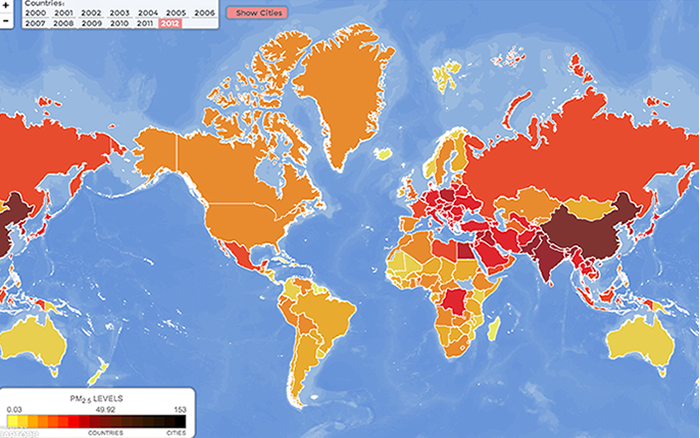
\includegraphics[width=\linewidth]{img/mappapm.png}
  \caption{Una mappa sul livello di particelle pm2.5}
  \label{fig:pollution_map}
\end{figure}


\subsection{I problemi della rappresentazione grafica}
Nonostante l’auto esplicabilità, il solo utilizzo della data visualization porta con sé diversi svantaggi. 
Il problema principale consiste nella totale assenza di feedback che un grafico offre al lettore.
\\
Prendiamo come esempio un grafico che mostra l'accumulo nel tempo delle polveri sottili nell'aria riempito con dati molto preoccupanti. 
Un utente, la cui preparazione sulla materia viene unicamente dalla legenda del grafico stesso, rischia di attribuire un peso sbagliato a quanto visualizzato.
\\ 
Un ulteriore problema della visualizzazione non animata, risiede nell'impossibilità di fornire all’interlocutore la percezione del tempo. 
Se ogni rilevazione di un grafico corrisponde ad una giornata differente; tramite le sole immagini risulta difficile comprendere quanto tempo richiedono dei processi come la risanazione dell'aria o lo spargimento delle polveri sottili.
\\ 
Infine, se dovessimo spostarci in un contesto ben più complesso dell’inquinamento atmosferico, come ad esempio un grafico astrofisico, è semplice pensare all’aumento della difficoltà nel rappresentare i dati. 
In questi contesti, seppure ancora un'ottima risorsa, la sola data visualization non è sufficiente per rendere delle informazioni comprensibili a non esperti.


%%%3%%%
\section{Sonificazione}
\subsection{Definizione di Sonificazione}
Con sonificazione si intende il processo tramite il quale dei dati di qualsiasi natura vengono trasformati in elementi acustici.
Più semplicemente, la sonificazione prende dei dati come input, e produce un suono come output \ref{fig:sonification_scheme}.
Il principio sul quale si basa questa tecnica è quello dell'auditory display, ovvero l'uso del suono per rappresentare delle informazioni.
La tecnica dell'auditory display risale a ben prima dell'informazione digitale, il semplice utilizzo di sirene e campane per attirare l'attenzione è solo uno dei possibili esempi.
Con il passare del tempo, questo principio ha trovato sempre più applicazioni nel settore dell'informatica, fino al 1992, anno nel quale è stato fondato l'International Community for Auditory Display (ICAD): il forum di ricerca più importante al mondo in questo campo.
Durante la sedicesima edizione dell'evento, il ricercatore Thomas Hermann, ha definito delle proprietà che ogni sistema di sonificazione deve possedere ~\cite{hermann}:
\begin{itemize}
  \item{il suono deve riflettere le proprietà dei dati rappresentati;}
  \item{la generazione del suono deve essere sistematica, i criteri tramite i quali il suono viene generato devono quindi essere chiari;}
  \item{la sonificazione deve essere deterministica, ovvero il suono prodotto deve essere sempre lo stesso per un dato input;}
  \item{il sistema deve essere riutilizzabile sia con gli stessi dati molteplici volte, sia con dati differenti.}
\end{itemize}
\begin{figure}[H]
  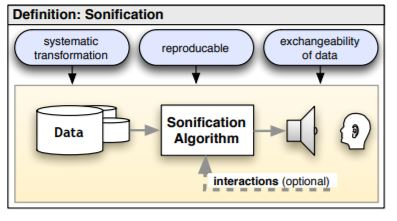
\includegraphics[width=\linewidth,scale=0.5]{img/schema.png}
  \caption{Lo schema riassuntivo della sonificazione}
  \label{fig:sonification_scheme}
\end{figure}


\subsection{L'utilizzo della sonificazione}
Il principale utilizzo della sonificazione è quello di fungere da alternativa alla data visualization, oppure arricchirla, tramite lo stimolo di un ulteriore senso: l’udito.
\\ 
Degli studi svolti sul campo della cinematografia e dell’intrattenimento in generale, sono arrivati alla conclusione che l’audio è la componente chiave per connettere lo spettatore con quello che sta vedendo. 
Uno dei metodi tramite i quali il cervello ritiene molto coinvolgente una rappresentazione grafica arricchita da una traccia audio consiste infatti nell’associazione di pattern visivi ad un certo suono.
In altre parole, il cervello è in grado di comprendere le informazioni uditive più semplicemente di quelle visive; l’orecchio infatti distingue meglio le tonalità di una traccia audio di quanto l’occhio riesca a leggere i vari colori ~\cite{audiovideo}.
\\
Con abbastanza inventiva, tramite la sonificazione è possibile trasformare qualsiasi informazione in suono, in questa tesi, ci concentreremo sui grafici.
Una semplice strategia per la sonificazione di un grafico consiste nell'associare un impulso sonoro tanto sgradevole quanto negativo sia il dato da rappresentare.
Tramite questa tecnica agli utenti risulterà molto più semplice interpretare quanto visualizzato.
\\ 
La sonificazione dei grafici è inoltre un ottimo modo per rappresentare i dati offrendo all’interlocutore una migliore percezione del tempo. In un grafico nel quale ogni rilevazione è identificata da una giornata differente, 
se associamo ad ogni dato una nota o, più in generale, un suono, all’utente risulterà sicuramente più semplice avere una migliore cognizione soggettiva del tempo trascorso.
\\ 
\subsubsection{Rappresentare dei dati multidimensionali}
Tramite la sonificazione, è semplice rappresentare in maniera chiara dei dati in forma multi dimensionale, come ad esempio, i grafici tridimensionali. 
Per rappresentarene le diverse proprietà di ogni dato nei grafici tridimensionali, è possibile associare a ognuna di queste uno dei vari aspetti dell'audio, come ad esempio il volume e la tonalità.
\subsubsection{La musica generativa}
La sonificazione può essere usata come strumento per la creazione di musica generativa.
Come ogni tipo di arte generativa, la musica generativa si riferisce alla creazione di una canzone in parte o totalmente da un sistema autonomo.
La caratteristica di questa tecnica è che il risultato non può essere ripetuto, in quanto infinito e sempre diverso.
In questo contesto, la sonificazione si presta molto bene per la creazione di musica, in quanto non segue i canoni della musica tradizionale.
Solitamente, una traccia sonificata, non distingue mai un inizio, una fine o un ritornello, ragione per la quale è possibile msuicare un flusso di dati potenzialmente infinito.

\subsection{Sonificazione ed accessibilità}
La sonificazione è un ottimo modo per rendere i dati accessibili ad individui portatori di disabilità visiva, come ad esempio, cecità completa o parziale.
Solitamente, le persone con disabilità visiva, per poter comprendere delle informazioni, si affidano a un terzo che legge per loro; spesso sotto forma di un software screen reader.
Questi software incontrano sempre grandi difficoltà nel leggere qualsiasi tipo di immagina, e quindi, anche i grafici.
La sonificazione risolve questo problema, permettendo al persona non vedente di comprendere le informazioni tramite la percezione uditiva, se affiancata ad una descrizione testuale leggibile da un screen reader ~\cite{accessibility}.
\\
La rappresentazione uditiva di è inoltre molto utile per le persone affette da daltonismo.
Alcune forme di data visualization utilizzano unicamente la simbologia dei colori per trasmettere informazioni; un possibile esempio legato al discorso dell'inquinamento consiste in una mappa dove ogni stato stato è colorato in base alla qualità dell'aria.
Affiancare ad ogni paese un determinato suono, oltre che un colore, rende la rappresentazione molto più comprensibile a persone affette da questa disabilità.

\subsection{Adattare un dato ad un formato sonoro}
Per creare una traccia audio coinvolgente, è possibile usare simultaneamente più aspetti dell'audio, i principali sono:
\begin{itemize}
  \item{il volume;}
  \item{la durata;}
  \item{la tonalità: quanto una nota è acuta;}
  \item{il timbro: cio che caratterizza il suono di uno strumento;}
  \item{la stereofonia: tramite l'utilizzo di due canali audio (ad esempio delle cuffie), è possibile creare un effetto di spazio e distanza tra i suoni.}
\end{itemize}
Le modalità di adattamento di un dato ad un formato sonoro sono solitamente stabilite dallo sviluppatore stesso, in base al formato dei dati a disposizione e al tipo di sensazione che si vuole trasmettere.
Vengono utilizzati principalemente tre approcci: la sintesi sonora, il design sonoro e la creazione di modelli di sonificazione.
\subsubsection{La sintesi sonora}
Se si vuole solamente fornire una rappresentazione alternativa a quella visiva, un'ottimo approccio per la creazione del suono è la sintesi sonora.
Con sintesi sonora si intendono le tecniche tramite le quali, con l'ausilio di hardware e software, un suono viene generato da zero, senza utilizzare strumentazione acustica.
Nel processo di sonificazione tramite sintesi, i dati vengono convertiti in una funzione periodica matematica.
Senza entrare troppo nel dettaglio, un possibile esempio di sonificazione tramite sintesi, consiste nell'ottenere l'onda sinusoidale più vicina ai punti in un grafico; le proprietà di quest'onda, quali frequenza e ampiezza, descrivono il suono che verrà prodotto.
\\
Una serie di dati, alternativamente, può essere trasformato in serie di campioni, comunemente chiamati wavetable.
Per suonare diversi toni musicali, vengono riprodotti i campioni audio ad intervalli regolari in base alla frequenza che si vuole ottenere.
Solitamente il numero di campioni utilizzati è 8192, un numero abbastanza alto da rendere riproducibile qualsiasi frequenza udibile dall'orecchio umano \ref{fig:wavetable}.
\begin{figure}[H]
  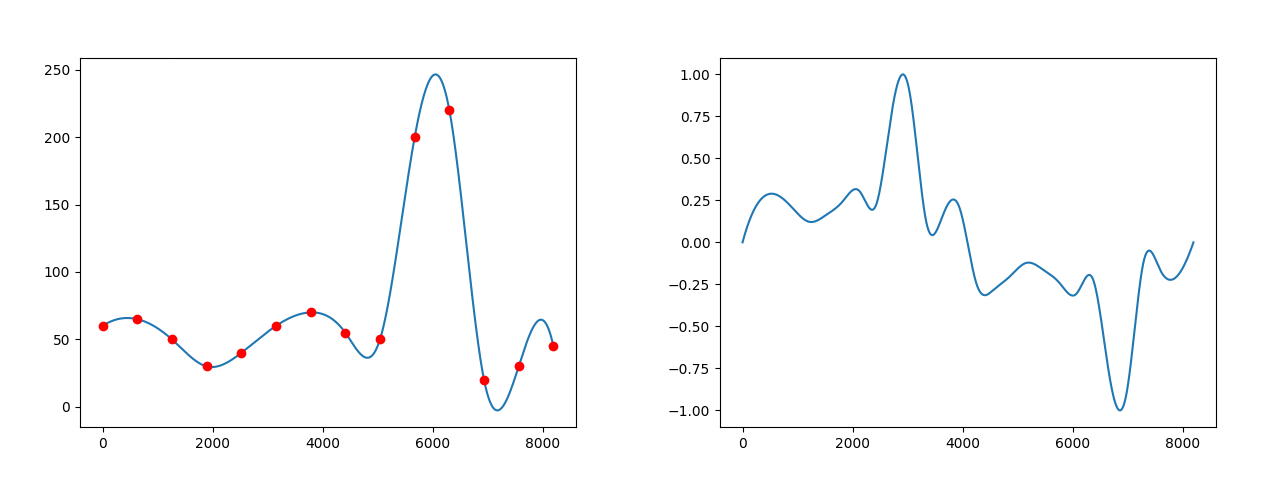
\includegraphics[width=\linewidth]{img/image.png}
  \caption{Una wavetable che ho generato a partire da dei dati sull'inquinamento.
  A sinistra, in rosso, sono raffigurate le rilevazioni dell'inquinamento. L'onda sonora periodica, mostrata a destra, è frutto dell'interpolazione, attenuazione e ripetizione di questi.}
  \label{fig:wavetable}
\end{figure}

 
Per quanto interessante, il suono creato con la sintesi è spesso poco espressivo.
La principale causa di questo fatto è la mancanza di armonici, ovvero le frequenze che si sommano alla frequenza fondamentale (quella che denomina la nota), solitamente responsabili per definire il timbro di uno strumento o di una voce umana.
\subsubsection{Design sonoro}
Un secondo possibile approccio consiste nell'utilizzare suoni di strumenti reali: un semplice esempio potrebbe coinvolgere l'utilizzo di suoni gradevoli e rilassanti per rappresentare dati positivi, e suoni sgradevoli per rappresentare dati negativi.
\\ Nel processo di sonificazione, si possono applicare inoltre nozioni di composizione musicale e design sonoro: l'andamento dei dati può essere infatti rappresentato dalle note di una scala, di un accordo o di qualsiasi altra forma di melodia.
La teoria musicale insegna inoltre a fare provare delle determinate emozioni all'ascoltatore; gli accordi e le scale maggiori esprimono emozioni positive, mentre le tonalità minori esprimono emozioni negative.
Se invece volessimo indurre una sensazione di timore per rappresentare un dato particolarmente negativo, potremmo utilizzare un suono molto forte e acuto, o, più in particolare, una dissonanza.
La dissonanza è un suono che non è in accordo con una scala musicale, risultando quindi fuori contesto e sgradevole.
Un designer sonoro può infine aggiungere alla propria traccia sonificata l'utilizzo di filtri e effetti audio digitali.
Tramite questi, è possibile ottenere un suono più ricco e complesso, che rispecchi meglio la natura dei dati.

\subsubsection{Model Based Sonification}
Un ultimo approccio di sonificazione, meno interessante dai due precedenti a livello implementativo, consiste nel creare modelli sonificativi.
Un modello di sonificazione è un sistema in grado di generare una risposta acustica quando un utente vi interagisce.
Per creare un modello, l'ideatore deve per prima cosa associare ad un evento ad una determinata azione, in seguito stabilire le modalità di interazione e infine procedere con la realizzazione.
A differenza della sintesi audio e del design sonoro, un modello è solamente in grado di rispondere a segnali esterni secondo regole predefinite, e non è in grado di generare suoni autonomamente.
Un esempio di modello di sonificazione è il theremin: uno strumento musicale elettronico tramite il quale un musicista, allontanando e avvicinando le mani alle antenne dell'oggetto, modifica la frequenza e l'ampiezza del suono prodotto ~\cite{sonification_model}.


\subsection{Esempi spiegati}
Il primo impiego effettivo della sonificazione risale al 1908. Lo studioso Hans Geiger si pose il problema di dare una rappresentazione immediata e di facile interpretazione della quantità di raggi gamma e particelle beta presenti nell’aria.
Inventò così il contatore Geiger: un dispositivo in grado di fornire un feedback sonoro in tempo reale sul livello di radiazione presente in un’area.
Il principio di sonificazione utilizzato nel contatore Geiger è molto semplice: lo strumento suona dei “click” ad intervalli regolari; più la concentrazione di radioattività è alta più il tempo di attesa tra i vari click si riduce.
\\\\
Con il passare del tempo, il concetto di sonificazione si è adattato a rappresentare dati di ogni natura, e non solo quelli legati a proprietà fisiche, diventando a tutti gli effetti una alternativa alla visualizzazione grafica.

\subsubsection{Sonificare il prezzo di Bitcoin}
\begin{figure}[H]
  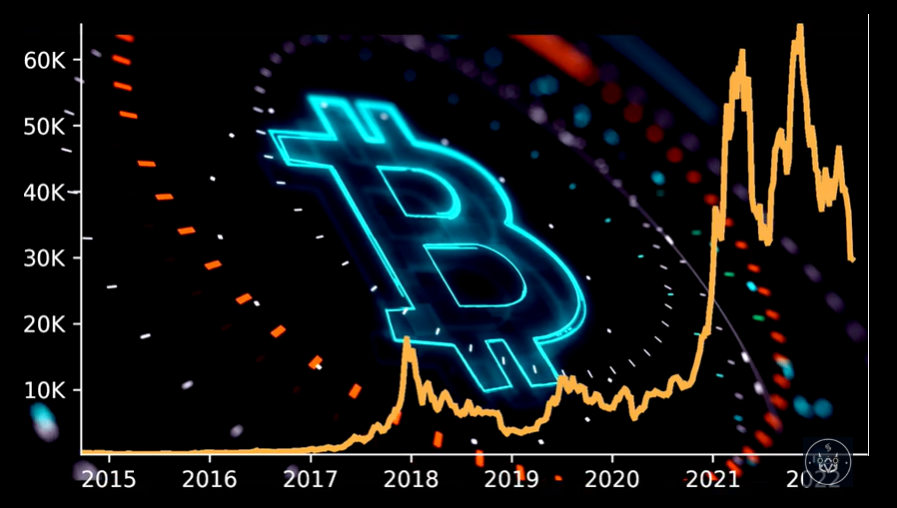
\includegraphics[width=\linewidth]{img/btc.PNG}
  \caption{L'andamento del prezzo del bitcoin tra il 2015 e il 2022, rappresentato con un grafico azionario.}
  \label{fig:btc}
\end{figure}
Il grafico in figura \ref{fig:btc}, è stato sonificato dal data scientist Rohith Teja.
Questo esperimento si differenzia da molti altri per la particolare gradevolezza del suono prodotto, anche ad un orecchio non esperto.
Per raggiungere questo scopo, il lo studioso ha utilizzato la sonificazione solamente per generare la sequenza di note; associando ad ogni variazione di prezzo del bitcoin una nota musicale.
Il suono vero e proprio è prodotto da dei sintetizzatori virtuali anni 80', all'interno di una Digital Audio Workstation: un software professionale per la produzione musicale.
Come base musicale Rohith ha scelto un'armonia di do maggiore, ovvero un set di note che possono essere suonate insieme.
Ogni dato presente nel grafico è mappato su una nota dell'armonia con un criterio molto semplice: più il prezzo del bitcoin è alto, più la nota è acuta.
E' stato utilizzato un insieme di note molto armonioso data la positività dei dati rappresentati ~\cite{bitcoin}.
\\\\


\subsubsection{Trasformare un'immagine in campioni audio}
Vediamo invece un esempio che utilizza la sintesi audio.
\begin{figure}[H]
  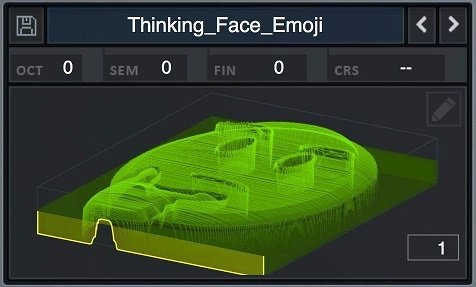
\includegraphics[width=\linewidth]{img/wavetable_emoji.jpg}
  \caption{La rappresentazione sonora di un emoji.}
  \label{fig:emoji_wavetable}
\end{figure}

Nell'immagine \ref{fig:emoji_wavetable}, viene mostrate una delle funzioni messe a disposizione dall'Xfer Serum, un sintetizzatore virtuale.
Questa feature permette di sonificare qualsiasi immagine importata nel programma secondo vari criteri.
Il criterio più semplice consiste per prima cosa nel convertire l'immagine in scala di grigi, e di ridimensionarla in un quadrato di dimensioni prefissate.
A partire da ogni riga dell'immagine viene poi generata una sequenza di campioni, ognuno dei quali mappato sul livello di luminosità del singolo pixel.
Tramite questo processo è possibile dare una rappresentazione sonora ad immagini come radiografie, fotografie di satelliti o rilevazioni di sensori ~\cite{serum}.

\subsubsection{Sonificare la volta celeste}
Durante la ricerca, le sonificazioni che più ho apprezzato riguardano la rappresentazione sonora dello spazio.
La cosa in comune tra questi esperimenti è la loro capacità di trasmettere un senso di grandezza e di infinità, accentuato dall'utilizzo del riverbero: l'effetto acustico ottenuto simulando la riflessione del suono in un ambiente. 
Sul sito della NASA, sono disponibili molti esempi di sonificazione di dati astronomici, ognuno dei quali utilizza approcci differenti.
Analizzando, ad esempio, la galassia NGC 1569, i ricercatori hanno deciso di rappresentare i tre colori principali dell'immagine con tre intervalli di frequenza differenti; in aggiunta, il livello di luminosità determina il volume di ogni suono.
Grazie questa strategia, è possibile distinguere, sia od occhio che a orecchio, i vari corpi celesti presenti nell'immagine.
Questa sonificazione utilizza un approccio bottom-top, consiste ovvero nel trasformare ogni riga dell'immagine in un suono e di concatenare questi in sequenza ~\cite{nasa}. 


	\clearpage{\pagestyle{empty}\cleardoublepage}
\chapter{Design e Tecnologie}                %crea il capitolo
%%%%%%%%%%%%%%%%%%%%%%%%%%%%%%%%%%%%%%%%%imposta l'intestazione di pagina

Questo capitolo è dedicato alla presentazione del design e delle tecnologie utilizzate per la realizzazione del progetto.
Nelle apposite sezioni, saranno approfondite le caratteristiche di ciascuna tecnologia, in modo da offrire una panoramica completa sulle scelte implementative effettuate.


\section{Definizione dei Requisiti}
Vengono riportati di seguito i requisiti definiti in fase di progettazione, questi si dividono tra requisiti funzionali e requisiti non funzionali.
\subsection{Requisiti funzionali}
I requisiti funzionali definiscono il comportamento e le funzionalità del sistema \cite{requisiti}.
I requisiti individuati sono:
\begin{itemize}
    \item[RF1]: L'applicativo deve mostrare lo stato dell'inquinamento dell'aria in tempo reale;
    \item[RF2]: L'applicativo deve permettere all'utente di navigare su una mappa, compresa di funzionalità di ricerca e zoom;
    \item[RF3]: L'utente deve essere in grado di ascoltare una simulazione audio relativa all'inquinamento di qualsiasi parte del mondo, in qualsiasi data;
    \item[RF4]: Molteplici sonificazioni degli stessi dati devono risultare nella medesima traccia audio;
    \item[RF5]: Insieme allaf traccia audio sonificata deve essere mostrato un grafico progressivo raffigurante l'andamento dell'inquinamento;
    \item[RF6]: Il sistema deve funzionare su qualsiasi dispositivo e sistema operativo.
\end{itemize}

\subsection{Requisiti non funzionali}
I requisiti non funzionali definiscono le caratteristiche del sistema che non sono direttamente legate alle sue funzionalità.
Non sono solitamente richieste dal cliente e si rispecchiano nelle scelte laterali di progettazione e sviluppo \cite{requisiti}.
I requisiti non funzionali individuati sono:
\begin{itemize}
    \item[RNF1]: Il sistema deve essere semplice ed intuitivo da utilizzare;
    \item[RNF2]: L'applicativo deve astrattizzare qualsiasi riferimento alla sintesi audio e alla teoria musicale;
    \item[RNF3]: L'applicativo deve essere in grado di produrre una sonificazione in tempi relativamente brevi.
\end{itemize}



\section{Progettazione grafica}
In seguito alla definizione dei requisiti, sono passato alla fase di progettazione grafica.
\subsection{Mockup}

\begin{figure}[h]
    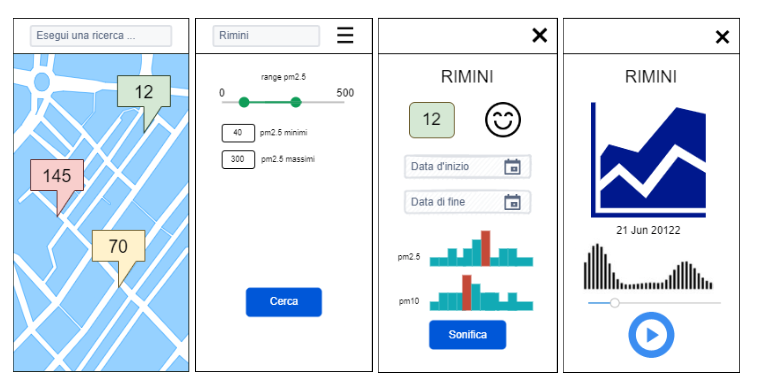
\includegraphics[width=\linewidth]{img/mockup.png}
    \caption{I mockup iniziali per la visualizzazione mobile}
    \label{fig:mockup}
\end{figure}

In Figura \ref{fig:mockup} sono riportati i mockup iniziali per la visualizzazione mobile dell'applicazione.
Per realizzare i mockups ho utilizzato la piattaforma online draw.io.
\begin{itemize}
    \item \textbf{Screen 1}: modella la prima view che viene mostrata, ogni pin rappresenta una stazione di rilevazione e il relativo indice di inquinamento in tempo reale. Al tap della casella di testo in alto viene aperta la view relativa a (Screen 2);
    \item \textbf{Screen 2}: In questa schermata l’utente può personalizzare la ricerca, mostrando solamente pin con inquinamento in un certo range, e spostare la camera sulla località selezionata;
    \item \textbf{Screen 3}: Al tap di un pin sulla mappa presente in (Screen 1), viene aperta la view relativa a (Screen 3). In questa schermata l’utente potrà selezionare l’intervallo di date il cui inquinamento rilevato verrà sonificato. Una volta selezionate le date, nei grafici sottostanti viene mostrata un’ anteprima dell’andamento delle rilevazioni nei giorni;
    \item \textbf{Screen 4}: Alla pressione del bottone Sonifica, viene mostrata la view relativa a (Screen 4), nella quale è presente un grafico che, tramite cambiamenti in tempo reale, accompagna la traccia audio generata a partire dai dati.
\end{itemize}

I mockup per la visualizzazione desktop non differiscono molto da quelli mobile, la mappa occupa l'intera pagina e le impostazioni per la sonificazione sono mostrate in un menu laterale a scomparsa \ref{fig:desktopmockup}.
\begin{figure}[H]
    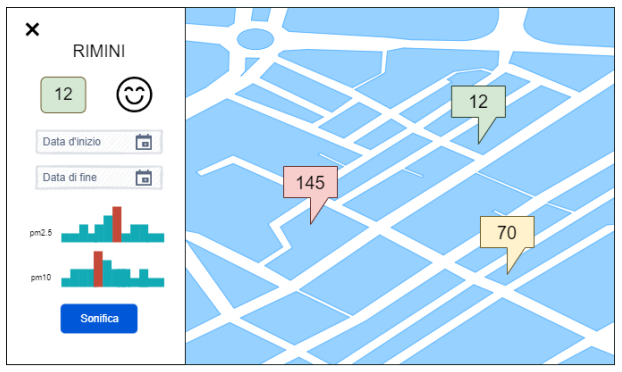
\includegraphics[width=\linewidth]{img/desktopmockup.PNG}
    \caption{I mockup iniziali per la visualizzazione desktop.}
    \label{fig:desktopmockup}
\end{figure}




%%%%%%%%%%%%%%%%%%%%%%%%%%%%%%%%%%%%
\section{Tecnologie web utilizzate}
L'idea di questo progetto nasce dalla necessità di fornire una rappresentazione della qualità dell'aria che respiriamo differente da quella solamente grafica.
Per questo fine ho deciso di sviluppare un'applicazione web: la risorsa informatica più facilmente accessibile ed utilizzabile.
A differenza di un'applicazione nativa, infatti, le webapp sono fruibili tramite browser da qualsiasi dispositivo connesso ad internet, senza bisogno di download o installazione \cite{appdiffs}.
Per comodità, ho suddiviso il programma in più parti: una parte di frontend, tramite la quale l'utente interagisce, e una parte di backend, che si occupa della sonificazione vera e propria.
In questa sezione verranno approfondite le tecnologie utilizzate per lo sviluppo del front end.

\subsection{HTML}
La pagina fruibile dall'utente presenta una struttura base HTML (Hyper Text Markup Language), un linguaggio per la formattazione di pagine web.
HTML è un linguaggio di pubblico dominio, la cui sintassi è stabilita dal World Wide Web Consortium (W3C): un'associazione non governativa che si occupa di diffondere l'accessibilità della rete e di standardizzare le tecnologie web.
La sintassi di HTML è composta da tag in cascata, i quali, letti dal browser, contengono le informazioni necessarie per l'impaginazione.

\subsection{CSS}
Il solo utilizzo di HTML non è sufficiente per ottenere un'interfaccia grafica gradevole e funzionale.
Per questo motivo ho utilizzato CSS (Cascading Style Sheet), un linguaggio utilizzato per definire lo stile di una pagina web, anch'esso reso standard da W3C da un insieme di regole.
CSS permette di attribuire stile grafico ai vari tag HTML, come ad esempio cambiare il colore di sfondo, la dimensione del testo e la posizione degli elementi.

\subsection{JavaScript}
Ho utilizzato Javascirpt per definire il comportamento della pagina in seguito alle interazioni dell'utente.
Javascript è un linguaggio di programmazione orientato ad eventi, interpretato durante l'esecuzione da un browser.
Javascript è comunemente utilizzato per introdurre effetti dinamici e funzionali chiamati eventi, invocabili dall'utente interagendo con la pagina HTML.
Ho scelto questo linguaggio per la sua semplicità nel gestire le richieste web, e per la sua ottima compatibilità con i vari browser.

\subsection{Jquery}
Spesso, collegare i tag HTML agli eventi definiti in Javasctipt, è un processo che, seppure non complicato, riempie il codice di debito tecnico.
Per questo ho delegato le interazioni tra le due tecnologie a Jquery: una libreria Javascript reperibile gratuitamente online.

\subsection{Bootstrap}
Bootstrap è una libreria di CSS disponibile gratuitamente, molto diffusa tra le applicazioni web.
Seppure questo framework si presti ottimalmente alla creazione di grafiche moderne e accattivanti, ho preferito limitarmi ad utilizzarlo per semplificare la gestione del layout della pagina, in particolare,
la posizione di elementi quali la mappa e il player video multimediale.

\subsection{Plotly}
Plotly è una libreria Javascript gratuita per la creazione di grafici.
Ho utilizzato questa libreria per creare i grafici che mostrano l'andamento dell'inquinamento nell'intervallo di tempo selezionato dall'utente.
Nonostante la libreria offra moltissimi stili di grafici, ho preferito utilizzare il grafico a barre, in quanto ritengo sia il più adatto per rappresentare questo tipo di dati.
Lo stile che ho deciso di applicare al grafico riprende i colori selezionati per lo standard AQI \ref{tab:aqi}. Ogni rilevazione viene colorata in base al livello di inquinamento.

\subsection{Leaflet - OpenStreetMap}
Ho utilizzato questi moduli per inserire una mappa interattiva all'interno della pagina web.
Leaflet è una libreria JavaScript open source per la gestione di mappe, facilmente estendibile e con una sintassi ad eventi simile a JQuery.
Per quanto riguarda invece l'aspetto della mappa ho applicato un layout vettoriale fornito da OpenStreetMap: un progetto open source sulla rappresentazione cartografica della superficie terrestre.
Tramite queste due componenti, l'utente può ingrandire la mappa e posizionare marker a proprio piacimento.
Siccome i colori utilizzati da EPA per l'AQI \ref{aqi} sono particolarmente chiari, ho applicato lo stile scuro, per aggiungere un contrasto maggiore.

\subsection{Esri Leaflet}
Al fine di permettere all'utente di eseguire ricerche per indirizzo e località, e reperire le informazioni di qualsiasi luogo alla pressione sulla mappa, ho utilizzato la libreria Esri Leaflet.
Esri Leaflet è una libreria JavaScript open source per la gestione dei dati geografici distribuita da Esri, un'azienda specializzata in questo campo.
Le funzionalità che ho utilizzato principalmente sono il geocoding e il reverse geocoding, ovvero la ricerca di coordinate geografiche a partire da un indirizzo e viceversa.

\subsection{AQIcn API}
Per ottenere i dati relativi alla qualità dell'aria da posizionare sulla mappa, ho utilizzato l'API di AQIcn.
Una API (applicaztion program interface), è un insieme di funzioni e procedure che, fungendo da interfaccia, permettono di interagire con un software esterno \cite{api}.
Questo servizio è stato messo a disposizione dal team del World Air Quality Index: un progetto no-profit che mira alla sensibilizzazione delle persone sulla tematica dell'inquinamento atmosferico.
AQIcn è un'implementazione di questo progetto, che fornisce agli sviluppatori, o ai soli interessati, dati trasparenti e aggiornati sulla qualità dell'aria in tempo reale.

\subsection{Weatherbit.io}
Purtroppo, al momento della progettazione e scelta delle tecnologie, l'API di AQIcn non metteva a disposizione una funzione per ottenere lo storico dei dati.
Per questo motivo, ho dovuto ricorrere ad una seconda API: Weatherbit.io.

\subsection{Javascript Fetch API}
Per rendere comunicanti la parte di frontend, la parte di backend e le varie API, ho utilizzato la funzioni Fetch messa a disposizione da javascript.
Tramite una chiamata Fetch, è possibile inviare una richiesta HTTP ad un server, e, se necessario, ricevere risposta.
Una chiamata a aquesta funzione permette di personalizzare la richiesta in base alle esigenze e al protocollo utilizzato; specificando l'URL di destinazione, modificando l'header e il body della richiesta, e gestendo la risposta.
Le chiamate a Fetch sono svolte in maniera asincrona; dove necessario ho utilizzato la caratteristica sintattica await per mantenere il flusso di esecuzione, aspettando il completamento della chiamata prima di proseguire.

\subsection{Python FastAPI}
Il software di backend che si occupa di gestire le richieste HTTP e fornire loro risposta è realizzato in Python.
Ho scelto questo linguaggio per la sua semplicità nella manipolazione di complesse strututre dati, e per l'enorme quantità di funzionalità matematiche offerte.
La libreriea utilizzata per elaborare le richieste di rete è FastAPI.
Tramite FastAPI è possibile creare un server web in maniera veloce, utilizzando parole chiave comuni nella sintassi di python.
Il software prodotto è una Restful API: un programma che utilizza il protocollo HTTP per ricevere e fornire dei dati \cite{api}.
Siccome il processo di sonificazione non è istantaneo, ogni richiesta viene gestita indipendentemente dalle altre, rendendo il server asincrono.




%%%%%%%%%%%%%%%%%%%%%%%%%%%%%%%%%%%%
\section{Tecnologie utilizzate per la sonificazione}

La software componente che esegue la sonificazione vera e propria è realizzata in Python in uno script differente da quello del server.
Il server, quando richiesto, esegue questo script passandogli come argomento tutti i dati necessari per produrre la traccia.
I dati inviati sono sotto forma di JSON, un formato standardizzato perticolarmente adatto all'interscambio di dati in rete.
I dati ricevuti dallo script di sonificazione sono: 
\begin{itemize}
    \item \textbf{data}: array di interi relativi alle varie rilevazioni;
    \item \textbf{days}: array di DateTimes, variabili rappresentanti l'orario e la giornata di ogni rilevazione;
    \item \textbf{index}: l'indice delle varie rilevazioni, può essere AQI, PM2.5 e PM10.
\end{itemize}
Questo programma svolge diversi compiti in successione, questi sono: ricevere i dati, creare le varie traccie, unirle in un'unico file wav, generare un'animazione in .gif, unire audio e video.

\subsection{Strategia di sonificazione}
Per sonificare i dati, ho utilizzato un approccio misto, sfruttando sia la sintesi audio che il design sonoro, approfonditi nel capitolo precedente.
Prima di progettare il sistema sonificativo, ho individuato le caratteristiche dei dati che volevo rappresentare:
le componenti di maggiore importanza sono l’andamento temporale dell'inquinamento e l'inquinamento residuo.
\subsubsection{L'andamento dell'inquinamento}
L'andamento temporale è rappresentato dalle varie rilevazioni nel tempo, siccome è un valore che tende a cambire rapidamente nel tempo, ha richiesto un approccio di sonificazione dinamico.
La scelta delle note utilizzate per rappresentare questo dato è molto semplice: più il valore dell'inquinamento è alto, più la nota è grave.
\subsubsection{L'inquinamento residuo}
L'inquinamento residuo consiste nel valore di rischio per la salute che si protrae nel tempo in seguito ad una giornata particolarmente inquinata.
A differenza della rilevazione AQI vera e propria, i cui valori possono variare drasticamente da un momento all'altro, l'accumulo di residuo si distingue in fasi di crescita e di diminuzione, in funzione a come si è comportato l'inquinamento nel corso della giornata \cite{residue}.
Per le fasi di crescita ho usato delle note veloci che si alzano di tonalità, mentre per la fase di diminuzione le stesse note sono ripetute con meno frequenza, e tendono ad abbassarsi nel tempo.
\subsubsection{Gestire il volume}
Un aspetto molto rilevante che ho attribuito a queste due traccie sta nella miscela dei loro volumi: più il valore dell'inquinamento tende ad alzarsi, più il suo volume si abbassa per lasciare spazio alla traccia dell'inquinamento residuo, che invece tende a crescere.
\subsubsection{L'applicazione della teoria musicale}
Per accentuare l'effetto della crescita e della diminuzione dell'inquinamento residuo, le note della traccia seguono una scala: più l'inquinamento è alto più le note sono acute.
Ho deciso di utilizzare una scala maggiore. Siccome le tonalità maggiori sono note per la loro positività, ho introdotto delle dissonanze in base al peggioramento della qualità dell'aria, volte a spezzare questa armonia.
Una dissonanza è una nota “fuori contesto” rispetto alla scala o all'accordo che si sta suonando; se inserita all'interno di una scala maggiore, sempre positiva e armoniosa, la dissonanza crea un effetto improvviso di tensione \cite{dissonance}.
Ho posto le dissonanze ad intervalli regolari nella scala in base al livello di inquinamento: più questo è alto, più le dissonanze sono frequenti e di maggior intensità.


\subsection{Design audio}
\subsubsection{I file MIDI}
Per quanto riguarda la parte di design audio, ho deciso di generare un file MIDI.
Il MIDI (Musical Instrument Digital Interface) è uno standard di comunicazione sviluppato agli inizi degli anni 80', è tutt'ora vastamente usato nel mondo della produzione musicale per la sua semplicità e la sua portabilità.
Tramite questo protocollo, è possibile comunicare gli stessi dati sia a software musicali che a dispositivi hardware, come tastiere e sintetizzatori, che li traducono in suoni \cite{midi}.
La creazione, modifica ed esportazione di tracciati MIDI è molto semplice in quanto non richiede alcuna conoscenza di linguaggi di programmazione e funzionamento del suono a livello hardware e software.
In aggiunta, la manipolazione della sequenza di note, è un processo incredibilmente più semplice e intuitivo rispetto alla modifica del segnale audio vero e proprio.
Una sequenza MIDI è una sequenza di eventi che si differenziano per la loro funzione; un evento ha un tempo di inizio, un tempo di fine, un canale e un valore.
Per misurare il tempo, i software musicali utilizzano vare metriche: battute di pentagramma, millisecondi, o tick MIDI.
Di default, un tick MIDI equivale a 1/960 di una battuta di pentagramma, il tempo è di 4/4 e la velocità è di 120 bpm \cite{midi}.
I principali eventi sono:
\begin{itemize}
    \item \textbf{Note On}: indica l'inizio di una nota, quando un tasto sulla tastiera viene premuto;
    \item \textbf{Note Off}: indica la fine di una nota, quando un tasto sulla tastiera viene rilasciato;
    \item \textbf{Control Change}: indica un cambiamento di stato, come ad esempio il cambio di tonalità di una nota mentre suona;
    \item \textbf{Program Change}: indica un cambio di strumento;
    \item \textbf{Meta Event}: indica un evento generale, può essere un messaggio di testo o un cambio di tempo.
\end{itemize}
Una sequenza MIDI può essere creata da uno strumento munito di tastiera, o da una Digital Audio Workstation: un software di produzione musicale; in particolare, queste ultime, presentano un'interfaccia sempre più incentrata sull'utilizzo di questo standard.
Lo strumento digitale più adatto alla composizione del MIDI è il piano roll: un editor che permette di visualizzare le note in un piano virtuale \ref{fig:pianoroll}. 
Nel piano roll, ogni nota è rappresentata da una casella, la sua posizione orizzontale indica il tempo in cui inizia, mentre la sua posizione verticale indica la tonalità.
\begin{figure}[H]
    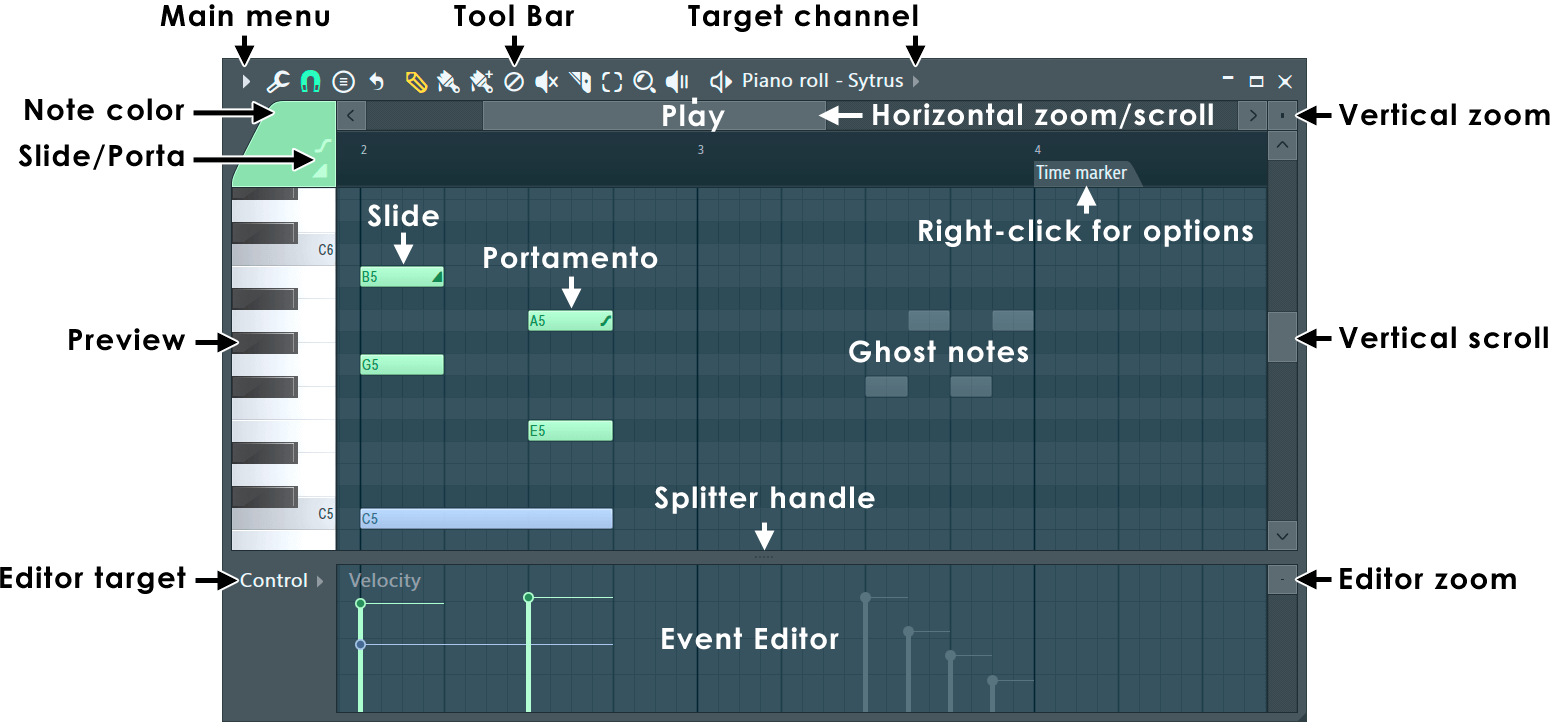
\includegraphics[width=\linewidth,scale=0.2]{img/pianoroll.png}
    \caption{Il piano roll di un software Digital Audio Workstation \cite{pianoroll_img}.}
    \label{fig:pianoroll}
\end{figure}
Lo standard MIDI, infine, comprende GeneralMidi: un'enumerazione di strumenti ed effetti audio.
Questa caratteristica mi ha permesso di concentrarmi solamente sulla scelta degli strumenti General MIDI e sulla generazione della sequenza di note, delegando la sintesi vera e propria ad un software terzo.
Per la creazione di file MIDI ho utilizzato MidiUtils, una libreria per Python che permette di creare un file MIDI specificandone i vari eventi.
Per la sintesi del file MIDI, invece, ho utilizzato Timidity++, un software open source che permette di sintetizzare un file MIDI in un file wav.
\subsubsection{Effetti audio VST3}
Per aggiungere spessore alle traccie midi sintetizzate, ho deciso di applicarvi degli effetti audio.
Scrivere effetti audio con risultati di qualità è un processo complesso, che richiede una conoscenza approfondita della propagazione del suono.
Per questo motivo, ho importato nel programma degli effetti audio sviluppati da professionisti.
La tecnologia che ho scelto è VST3 (Virtual Studio Technology 3), un formato che standardizza l'interfaccia tra il plugin e il software che lo utilizza.
Il formato VST è stato introdotto da Steinberg nel 1996 nel suo software Digital Audio Workstation Cubase \cite{vst3}. Insieme allo standard è stato inoltre sviluppato un SDK (Software development kit), ciò ha permesso a molti programmatori
di avvicinarsi al mondo della programmazione di effetti audio ed audio processing, donando notorietà al formato.
Per caricare un plugin VST3 in un software diverso da una Digital Audio Workstation ho utilizzato Pedalboard: una libreria per Python sviluppata da Spotify che internamente utilizza JUCE, un framework scritto in c++ per il processing audio.
Tramite un array contenente coppie chiave valore, è possibile impostare i parametri dell'effetto, e di seguito applicare questo ad un array di campioni audio da 32 bit.
\subsubsection{Archetype Gojira}
Gli effetti audio che ho scelto sono presenti nel Software Archetype Gojira: un plugin VST3 sviluppato da NeuralDSP insieme a Gojira, una band metal francese.
Seppure questo plugin sia stato sviluppato per simulare in tempo reale un amplificatore per chitarra, ho deciso di utilizzarlo solamente per gli effetti audio che mette a disposizione.
Gli effetti audio che ho applicato alle traccie sono i seguenti:
\begin{itemize}
    \item \textbf{Delay}: un effetto che, suonando più volte lo stesso input ad intervalli regolari, dona al suono un effetto di eco. Ho usato il delay per accentuare la persistenza del residuo di inquinamento nell'aria;
    \item \textbf{Reverb}: un effetto in grado di simulare i rimbalzi delle onde sonore in una stanza;
    \item \textbf{Shimmer}: un effetto che, preso come input un suono, ne riproduce un'armonizzazione, creando un effetto di coro a molte voci.
\end{itemize}

\subsection{Sintesi audio}
La sintesi audio è stata utilizzata per sonificare la forma del grafico, negli intervalli nei quali il livello di inquinamento supera la soglia di totale salubrità.
La traccia che ho assegnato alla sintesi audio è il Sub-bass, ovvero dei toni profondi le cui frequenze scendono sotto i 70 Hz; in questo range di frequenze, l'orecchio umano è solitamente meno sensibile, ragione per la quale il Sub-bass viene percepito piuttosto che ascoltato \cite{subbass}.
Per rappresentare un grafico sotto forma di audio, ho usato le wavetable, introdotte nel primo capitolo.
Le wavetable che ho composto hanno lunghezza fissa di 8192 campioni float da 32 bit ciascuno.
La forma dell'onda sonora risultante è strettamente legata alla forma del grafico, tramite questa strategia sono riuscito ad ottentere distinzione tra timbri nella traccia.
I campioni da riprodurre vengono scritti in un buffer che verrà in seguito unito alla traccia audio finale.
\subsubsection{Librerie utilizzate}
Lo script fa ampiamente uso delle librerie Numpy e Scipy, per la semplicità di utilizzo e la velocità di esecuzione.
In particolare, ho utilizzato Numpy per semplificare la manipolazione di array rappresentanti i campioni audio, e Scipy per la funzionalità di interpolazione periodica.
\subsubsection{LFO}
Per aggiungere più significato alla traccia sintetizzata ho assegnato al volume di questa un LFO (low frequency oscillator).
L'LFO consiste in un oscillatore a bassissima frequenza (sotto i 20 Hz). L'oscillatore è il componente base per la sintesi audio, viene usato per generare un'onda periodica con una certa ampiezza, frequenza e forma, solitamente sinusoidale, quadrata o triangolare \cite{izotope}.
L'onda creata dall'LFO non rappresenta una nota da ascoltare ma un segnale tramite il quale un'altra onda viene modulata.
In questo caso specifico, l'onda modifica il volume della traccia di Sub-bass in modo da creare delle variazioni oscillanti di ampiezza nel tempo, come mostrato in Figura \ref{fig:lfo}.
\begin{figure}[H]
    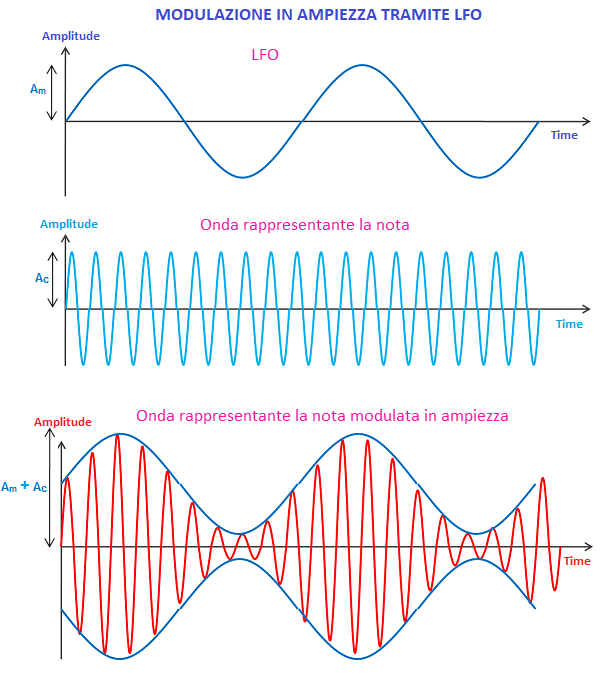
\includegraphics[width=\linewidth]{img/lfo.png}
    \caption{Un esempio di modulazione di ampiezza \cite{lfo_img}. I testi dell'immagine sono stati modificati per adattarli al contesto.}
    \label{fig:lfo}
\end{figure}
\subsubsection{Enveloper}
La sintesi audio porta con sè diversi problemi e complicazioni, la più comune tra queste è la presenza di un suono simile ad un “pop” durante la riproduzione.
Questi suoni sgradevoli sono causati suonando onde discontinue: quando lo speaker che riproduce l'audio, passando da una nota all'altra, percorre distanze troppo grandi in un tempo troppo breve.
Per evitare questo problema, ho utilizzato un Enveloper: un filtro che permette di gestire il volume in modo graduale.
L'enveloper è stato introdotto dall'ingegnere Robert Moog nel 1964, data la necessità di articolare il volume in maniera differente dai soli stati on/off.
I primi prototipi sviluppati di questo filtro caricavano e scaricavano lentamente dei condensatori attenuando il volume di conseguenza \cite{enveloper}.
Ad oggi, ogni sintetizzatore hardware e software mette a disposizione gli enveloper, la formula più comune è ADSR \ref{fig:asdr}, questo filtro gestisce l'andamento del volume in quattro stadi:
\begin{itemize}
    \item \textbf{Attack}: fase di crescita del volume, quando la nota viene premuta;
    \item \textbf{Decay}: fase di diminuzione del volume, la nota è ancora premuta, ma il volume diminuisce;
    \item \textbf{Sustain}: fase di mantenimento del volume, la nota è ancora premuta, il volume rimane stabile;
    \item \textbf{Release}: fase di diminuzione del volume, la nota viene rilasciata, il volume diminuisce.  
\end{itemize}
Siccome nel processo di sonificazione non vengono premuti effettivamente dei tasti, ho deciso di rimuovere le fasi di decay e sustain;
lo scopo dell'enveloper è stato quello di evitare il suono sgradevole citato precedentemente, aumentando e diminuendo il volume ad inizio e fine di una nota.
\begin{figure}[H]
    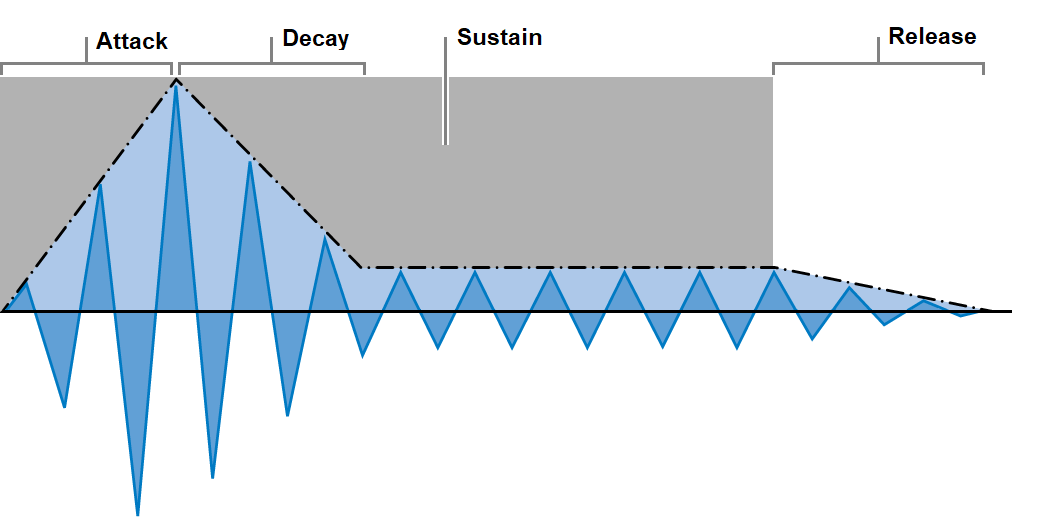
\includegraphics[width=\linewidth,scale=0.2]{img/adsr.PNG}
    \caption{Lo schema riassuntivo di un Enveloper ADSR \cite{env_img}.}
    \label{fig:asdr}
\end{figure}

\subsection{Creazione del video}
Per la generazione dell'animazione ho utilizzato matplotlib, una libreria di Data Visualization che permette di creare grafici.
In particolare, tramite \texttt{FuncAnimation} è possibile creare un'animazione a partire da una funzione che restituisce un grafico;
ogni rilevazione viene rappresentata da un frame, i quali vengono poi uniti in un unico file .gif ad intervalli di 0.5 secondi ciascuno.

\subsection{Unire Audio e Video}
L'aggiunta della traccia audio al file di animazione è stata possibile grazie a moviepy.
Moviepy è una libreria python per la manipolazione di video di diversi formati.
Per la funzionalità che ho utilizzato, moviepy richiama ffmpeg: una suite software cross platform per creare, tagliare, unire video.

\subsection{Altri software e hardware utilizzati}
\subsubsection{Ableton Live 10 Lite}
Ableton è una Digital Audio Workstation (DAW) che permette di registrare, modificare e riprodurre audio.
Ho utilizzato questo software in fase di prototipazione per comporre dei possibili risultati della sonificazione, applicare loro degli strumenti General MIDI e degli effetti audio.
Per la selezione delle note, ho utilizzato una tastiera compatibile con lo standard MIDI.
Durante la fase di testing, ho inoltre utilizzato Ableton per importare le traccie MIDI e gli audio sonificati, al fine di verificarne la correttezza.
\subsubsection{Audacity}
Audacity è un software open source per la manipolazione dell'audio.
Ho utilizzato questo software per analizzare in maniera più approfondita i campioni in fase di testing al fine di scoprire l'origine dei suoni sgradevoli.
Grazie alle funzione di zoom messa a disposizione è stato possibile individuare il problema con molta facilità.
\subsubsection{Visual Studio Code}
Visual Studio Code è un editor di testo open source, sviluppato da Microsoft.
Ho prediletto questo software per la sua semplicità di gestione di molteplici file simultaneamente, e per la sua completezza nelle funzionalità.
\subsubsection{Insomnia}
Insomnia è un software open source tramite il quale è possibile effettuare richieste HTTP e visualizzarne le risposte.
Ho utilizzato questo client in fase di test per comprendere la struttura delle risposte alle varie chiamate API effettuate.

\newpage
\section{Architettura del sistema schematizzata}
In Figura \ref{fig:uml} viene presentata una schematizzazione dell'architettura del sistema.
\begin{figure}[H]
    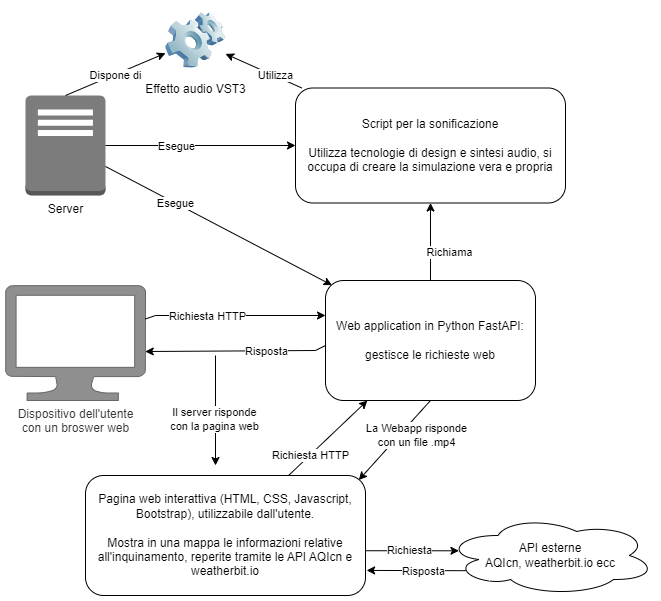
\includegraphics[width=\linewidth]{img/uml.png}
    \caption{L'Architettura del sistema.}
    \label{fig:uml}
\end{figure}
	\clearpage{\pagestyle{empty}\cleardoublepage}
\chapter{Implementazione}                %crea il capitolo
%%%%%%%%%%%%%%%%%%%%%%%%%%%%%%%%%%%%%%%%%imposta l'intestazione di pagina

Questo capitolo descrive le scelte implementative prese per la realizzazione dell'applicazione.
Il testo è arricchito da sezioni del codice sorgente, per facilitare la comprensione delle parti più complesse.

\definecolor{lightgray}{rgb}{.9,.9,.9}
\definecolor{darkgray}{rgb}{.4,.4,.4}
\definecolor{purple}{rgb}{0.65, 0.12, 0.82}
\lstdefinelanguage{JavaScript}{
  keywords={typeof, new, true, false, catch, function, return, null, catch, switch, var, if, in, while, do, else, case, break},
  keywordstyle=\color{blue}\bfseries,
  ndkeywords={class, export, boolean, throw, implements, import, this},
  ndkeywordstyle=\color{darkgray}\bfseries,
  identifierstyle=\color{black},
  sensitive=false,
  comment=[l]{//},
  morecomment=[s]{/*}{*/},
  commentstyle=\color{purple}\ttfamily,
  stringstyle=\color{red}\ttfamily,
  morestring=[b]',
  morestring=[b]",
  xleftmargin=-25pt,
  xrightmargin=-50pt,
  basicstyle=\scriptsize\sffamily
}

\section{Realizzazione della Mappa}
\subsection{Differenze con i mockup}
Durante lo sviluppo del progetto, ho apportato delle migliorie rispetto ai mockup.
Il cambiamento più significativo è stato quello di rimuovere i pin rappresentanti le varie stazioni a favore di una suddivisione in zone, ognuna delle quali delimitata da un cerchio colorato.
Il colore di ogni zona è definito dall'AQI medio mentre la grandezza dal numero di stazioni raggruppate.
Il centro di ogni cerchio è calcolato come punto medio da ogni stazione raggruppata.
Cliccando su un qualsiasi punto della mappa comparirà un pin con il nome della località, il valore AQI attuale e un grafico che mostra l'andamento della qualità dell'aria nelle ultime ore.
I pin possono essere aggiunti e rimossi in qualsiasi momento.
Premendo su un pin viene mostrato il menù a scomparsa per personalizzare la sonificazione.
Tralasciando qualche dettaglio grafico e di scelta dei colori, il menù è simile a quello presente nel mockup; una differenza volta a migliorare l'esperienza utente è stata quella di pre-impostare l'intervallo di tempo per la sonificazione a quello mostrato nel pin.
Al fine di permettere all'utente di effettuare più sonificazioni contemporaneamente, il player video è stato rimosso dalla pagina.
Ad ogni richiesta di sonificazione, viene mostrata in basso a destra una notifica cliccabile, che permette di aprire la simulazione in una nuova scheda del browser.
I colori utilizzati per i grafici, i cerchi e le notifiche riprendono quelli stabiliti dallo standard AQI \ref{tab:aqi}. La schermata finale è rappresentata in Figura \ref{fig:schermata}.
\begin{figure}[h]
  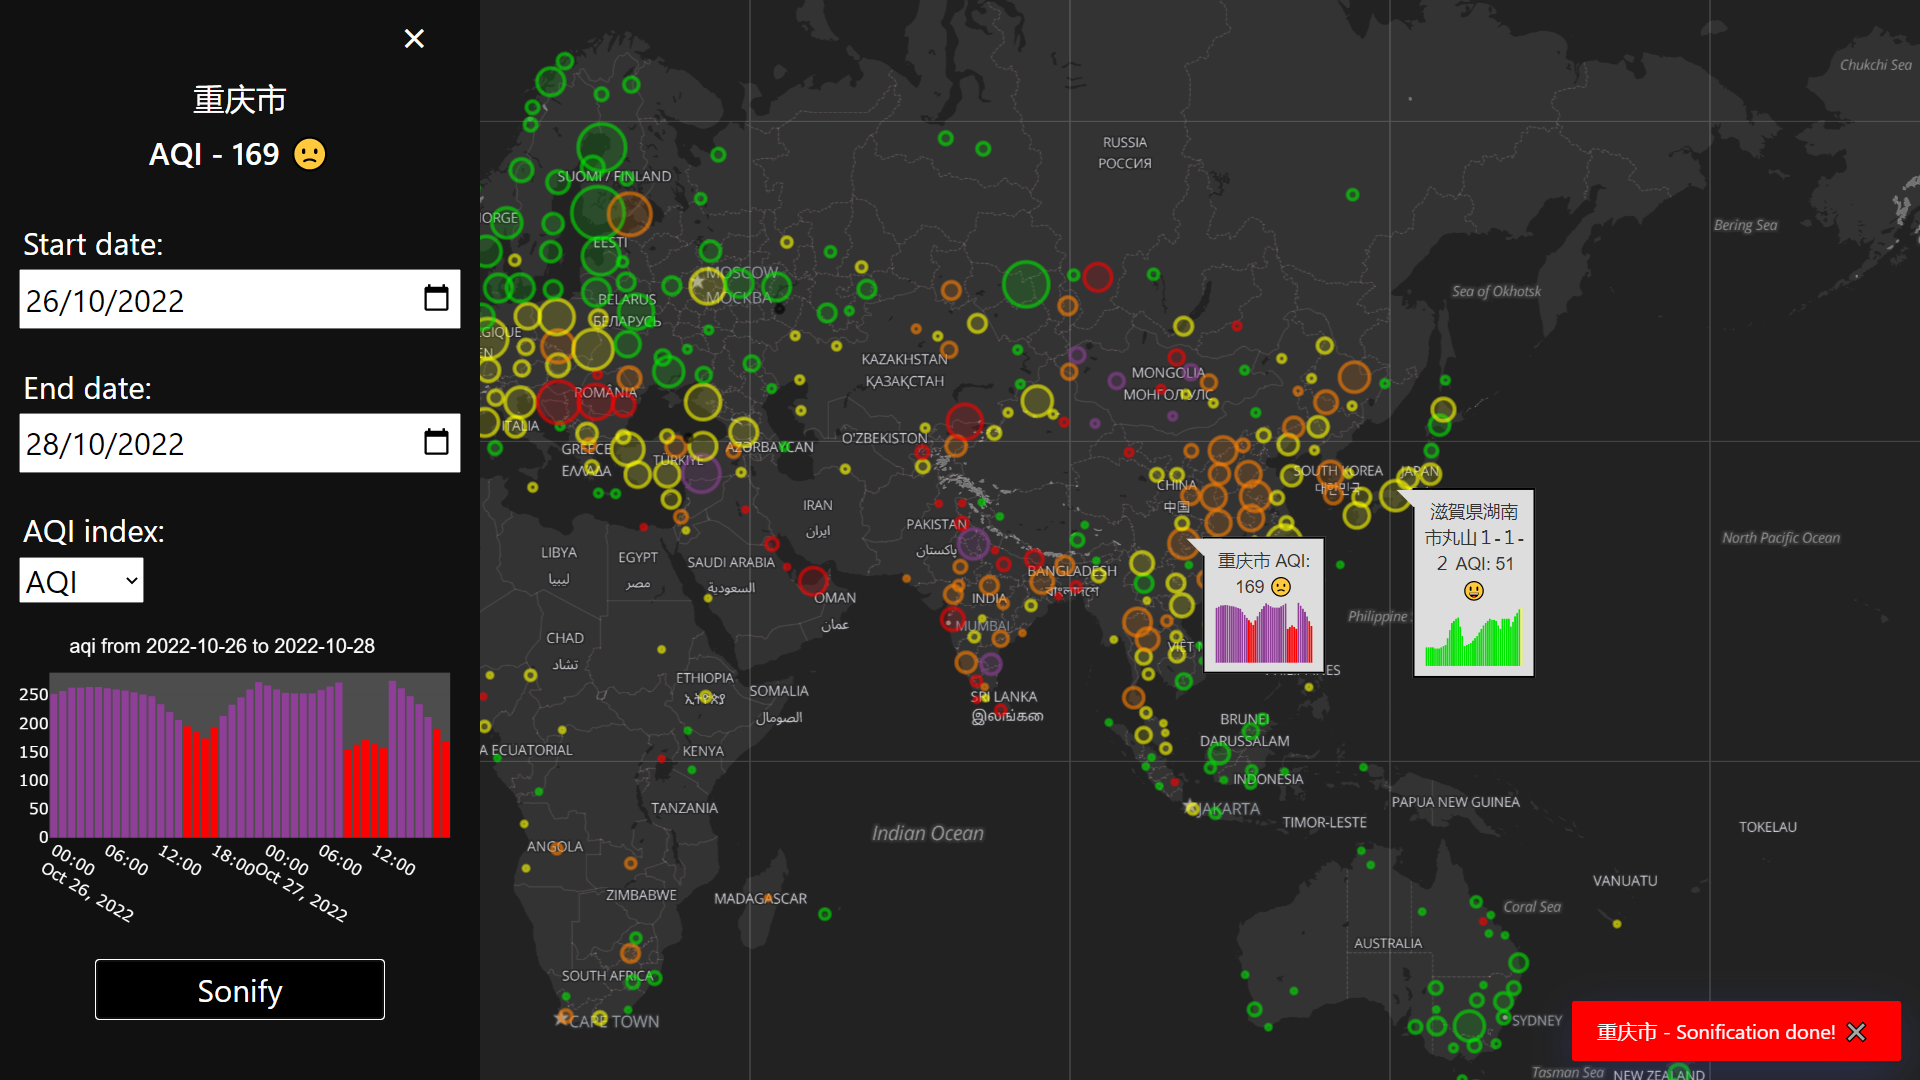
\includegraphics[width=\linewidth]{img/schermata.png}
  \caption{La schermata e le varie componenti}
  \label{fig:schermata}
\end{figure}
\subsection{Dettagli implementativi}
\subsubsection{Generazione dei cerchi}
La preparazione della schermata avviene in diverse fase consecutive.
Per prima cosa, tramite la libreria Leaflet, la mappa viene creata e visualizzata nella pagina.
Immediatamente dopo, tramite una chiamata all'API di AQIcn, vengono scaricati i dati relativi a tutte le stazioni di rilevazione presenti.
La visualizzazione delle zone circolari è affidata alla funzione load circles (listato ~\ref{lst:loadCircles}), che prende come unico parametro un oggetto JSON \cite{json}, contenente i dati delle stazioni.
La funzione divide il mondo in un totale di 4900 zone, 70 in altezza e 70 in larghezza, ognuna identificata da un indice univoco.
Per ogni stazione di ricerca, viene calcolato l'indice della zona a cui appartiene e viene inserita in un'apposita struttura dati.
\begin{lstlisting}[language=Javascript,caption={Suddivisione in zone delle stazioni.},label={lst:loadCircles}]
// get chunk unique index based on lat, lng
function get_chunk_idx(lat, lng, chunks_per_dim) {
    let lat_chunk = Math.floor((lat + 90) / 180 * chunks_per_dim);
    let lng_chunk = Math.floor((lng + 180) / 360 * chunks_per_dim);
    return lat_chunk * chunks_per_dim + lng_chunk;
}

// define chunk size
let chunks = {};
let chunks_per_dim = 70;   

// load chunks
for(let pin of data) {
    // ignore stations with no data
    if(pin.aqi == '-') continue;
    let lat = pin.lat;
    let lng = pin.lon;
    let chunk_idx = get_chunk_idx(lat, lng, chunks_per_dim);
    if(!(chunk_idx in chunks)) 
        chunks[chunk_idx] = [pin];
    else 
        chunks[chunk_idx].push(pin);
}
\end{lstlisting}
In seguito alla suddivisione in zone, per ognuna di queste viene calcolato il valore AQI e il punto medio delle stazioni raggruppate; 
in base a queste informazioni, viene disegnato un cerchio di colore e grandezza appropriati. Eventuali zone vuote vengono ignorate.


\subsubsection{Implementazione dei marker personalizzati}
Cliccando sulla mappa, viene eseguita la funzione map inspect (listato ~\ref{lst:mapInspect}).
Per prima cosa la funzione ottiene la latitudine e la longitudine del punto cliccato e, tramite reverse geocoding, ottiene il nome della località.
L'esecuzione passa in seguito alla funzione create marker che, da un set di coordinate e un nome, crea un marker personalizzato (listato ~\ref{lst:createMarker}).
La funzione si occupa, inoltre, di ottenere lo storico delle ultime rilevazioni AQI della zona, eseguendo una chiamata all'API di weatherbit.io, questi dati
vengono utilizzati in seguito per creare il grafico che compare nel pin.
Per rimuovere un pin, è sufficiente cliccare con il tasto destro del mouse, o effettuare una pressione prolungata se da mobile.
La struttura di un marker è un'estensione di quella default offerta da leaflet, sono state aggiunte le informazioni relative alla posizione geografica e all'ultima rilevazione AQI avvenuta, al fine di semplificare la gestione dei dati (listato ~\ref{lst:markerextension}).
\begin{lstlisting}[language=Javascript,caption={La struttura di un marker personalizzato.},label={lst:markerextension}]
// custom marker extension, values are placeholders
myAqiMarker = L.Marker.extend({
    options: {
        aqi: 0,       // last aqi value detected
        location: '', // location name
        lat: 0,       // latitude
        lng: 0        // longitude
    }
});
\end{lstlisting}

\begin{lstlisting}[language=Javascript,caption={La funzione map inspect.},label={lst:mapInspect}]
async function map_inspect(event) {

  // event consiste nelle informazioni relative all'evento di pressione sulla mappa
  let latlng = event.latlng;
  let lat = latlng.lat
  let lng = latlng.lng
  // reverse geocoding to get location name
  await geocodeService.reverse().latlng(event.latlng).run(async function (error, result) {

      // get address
      let add = result.address;
      let location = add.City || add.LongLabel;
      // add marker
      create_marker(lat, lng, location);

  });

}
\end{lstlisting}


\begin{lstlisting}[language=Javascript,caption={La funzione create marker.},label={lst:createMarker}]
async function create_marker(lat, lng, location) {
    
    // load history
    get_today_history(lat, lng).then(async(history) => {

        // get the history
        let id = String(Date.now());
        let aqis = await history.get_index('aqi');
        let time = await history.get_index('timestamp_local');
        let aqi = aqis[aqis.length - 1];

        new aqiMarker([lat, lng], {

            // custom marker label
            icon: L.divIcon({
                className: 'my-div-icon',
                html:
                    `<div class="speech-bubble">
                        ${location} AQI: ${aqi} ${get_emoji(aqi)}
                        <img class="aqi_preview" id="${id}"></img>
                    </div>`,
            }),
    
            // additional marker info
            location: location,
            aqi: aqi,
            lat: lat,
            lng: lng,
    
        }).addTo(layerGroup).on('click', load_offcanvas).on('contextmenu', function(e) { map.removeLayer(this); });
    
        // create graph inside the marker
        create_small_graph(aqis, time, id);

    });
    
}
\end{lstlisting}

\subsubsection{Utilizzare il geocoding}
All'utente è data la possibilità di ispezionare una località specificandone il nome, l'indirizzo o la posizione geografica.
La ricerca vera e propria è delegata all'API Esri di ArcGIS, che restituisce una lista di possibili risultati mostrati sotto la casella di testo.
Al click di uno di questi, dall'evento, viene estratto il nome del luogo, la latitudine e la longitudine, con questi parametri, viene chiamata la funzione map inspect, spiegata precedentemente.


\lstloadlanguages{Python}
\lstset{
  language=Python,
  basicstyle=\scriptsize\sffamily,
  stringstyle=\color[HTML]{933797},
  commentstyle=\color[HTML]{228B22}\sffamily,
  emph={[2]from,import,pass,return}, emphstyle={[2]\color[HTML]{DD52F0}},
  emph={[3]range}, emphstyle={[3]\color[HTML]{D17032}},
  emph={[4]for,in,def}, emphstyle={[4]\color{blue}},
  showstringspaces=false,
  breaklines=true,
  prebreak=\mbox{{\color{gray}\tiny$\searrow$}},
  xleftmargin=-25pt,
  xrightmargin=-50pt,
}

\subsubsection{Personalizzare la sonificazione}
Al click del marker, viene mostrato un menù a scomparsa che permette di personalizzare la sonificazione \ref{fig:schermata}.
I dati, quale il nome della località, l'intervallo di date iniziale e l'ultima rilevazione AQI effettuata, sono caricati direttamente a partire dal marker che ha chiamato la funzione.
Al cambiamento di ogni elemento presente nel form di personalizzazione è associato una funzione che valida i dati inseriti e, in caso di successo abilita il pulsante di conferma e aggiorna il grafico di anteprima (listato ~\ref{lst:formChange}).
In aggiunta, in caso di dati validi, le informazioni riguardanti la sonificazione vengono caricati in una struttura dati denominata sonification data, che verrà usata come payload della richiesta di sonificazione.

\begin{lstlisting}[language=Javascript,caption={La funzione che gestisce il cambiamento di un elemento del form.},label={lst:formChange}]
async function load_index(){

  // load useful data from form
  let start_date  = $("#offcanvas_start_date").val();
  let end_date    = $("#offcanvas_end_date").val();
  let lat         = $("#offcanvas_aqi").attr("data-lat");
  let lng         = $("#offcanvas_aqi").attr("data-lng");
  let index       = $("#offcanvas_index").val();
  
  get_history(lat, lng, start_date, end_date, index).then(async (history) => {

    let aqis = await history.get_index(index);
    let time = await history.get_index('timestamp_local');
    create_graph_image(aqis, time, "offcanvas_plot", `${index} from ${start_date} to ${end_date}`);
    $("#offcanvas_btn_sonify").show();

    sonification_data = {
      idx: index,
      data: aqis,
      days: time,
      location: $("#offcanvas_location").text()
    }

  }).catch(async (error) => {
      
    // if form data is invalid, or api call fails, hide sonify button
    $("#offcanvas_btn_sonify").hide();
    $("#offcanvas_plot").attr("src", "");
    console.log(error);

  });

}
\end{lstlisting}

\subsubsection{Gestire lo storico}
Lo storico delle rilevazioni AQI è gestito nel file aqi api.js.
Per ottenere lo storico, è necessario creare una nuova istanza della classe History, passando come parametri la latitudine e la longitudine della zona di interesse e l'intervallo di date (listato ~\ref{lst:history}).
Una volta ottenuto l'oggetto, tramite la funzione get index, è possibile ottenere un array contenente i valori di un indice di interesse, quali il PM10, il PM2.5, l'O3, ecc.
\begin{lstlisting}[language=Javascript,caption={La classe History.},label={lst:history}]
function History(lat, lng, start_date, end_date) {
    this.lat = lat;
    this.lng = lng;
    this.start_date = start_date;
    this.end_date = end_date;
}

History.prototype.load = async function() {
    let request = `https://api.weatherbit.io/v2.0/history/airquality?lat=${this.lat}&lon=${this.lng}&start_date=${this.start_date}&end_date=${this.end_date}&tz=local&key=${weatherbit_key}`;
    let response = await fetch(request);
    let resp_data = await response.json();
    this.data = resp_data.data;
}

History.prototype.get_index = async function(index) {
    let arr = this.data.map((item) => item[index]);
    return arr.reverse();
}
\end{lstlisting}

\subsubsection{Tutorial}
Al fine di migliorare la user experience, ho inserito un semplice tutorial che spiega come utilizzare l'applicazione.
Il tutorial consiste in dei messaggi che vengono mostrati nella parte inferiore dello schermo.
Ogni messaggio rimane in attesa del completamento di una determinata azione, al compimento di questa, il messaggio viene nascosto e viene mostrato il successivo.
Solo seguendo il tutorial, l'utente può effettuare la prima sonificazione.



\section{Implementazione del server}
Il server è in grado di ricevere richieste di tre tipi, in base al percorso di questa.
Per ottenere la pagina web interagibile, è possibile effettuare una richiesta GET al percorso / (root del server), da qualsiasi browser web.
Una volta selezionata la località, l'indice da sonificare, e l'intervallo di date, tramite il bottone sonifica viene eseguita una richiesta POST al percorso /sonify; i dati citati precedentemente sono inviati in formato JSON (listato ~\ref{lst:sonify}).
Questa richiesta richiama, in un processo secondario, lo script sonify.py; al suo completamento, il server legge i byte del file video generato e li restituisce al client.
Cliccando sulla notifica di avvenuta sonificazione, il client effettua una richiesta GET al percorso /video, che apre, in una nuova scheda, una schermata con il video riproducibile.

\begin{lstlisting}[language=Python,caption={La funzione che gestisce la richiesta /sonify.},label={lst:sonify}]
class SonifyRequest(BaseModel):
  # data array
  data:   list = Field(..., example=[121, 140, 150, 51, 67, 18])
  # dateTimes array
  days:   list = Field(..., example=["2021-01-01T00:00:00", "2021-01-01T00:00:01"])
  # data index (AQI, PM2.5, PM10)
  idx:    str 
\end{lstlisting}



\section{Sonificazione}
Di seguito vengono approfondite le scelte implementative per quanto riguarda la realizzazione della sonificazione vera e propria.
Le sezioni di codice successive fanno ampimente uso di due funzioni di utility, in grado di cambiare un valore da un intervallo di valori ad un altro (listato ~\ref{lst:utils}).

\begin{lstlisting}[language=Python,caption={Funzioni utility.},label={lst:utils}]
def map_value(value, in_min, in_max, out_min, out_max):
  # handles rare case where minium AQI and maximum AQI are the same
  if in_min == in_max:
      return (out_min + out_max) / 2
  return (value - in_min) * (out_max - out_min) / (in_max - in_min) + out_min

def map_value_int(value, in_min, in_max, out_min, out_max):
  return math.floor(map_value(value, in_min, in_max, out_min, out_max))
\end{lstlisting}



\subsection{Aspetti dell'inquinamento Sonificati}
Prima di progettare il sistema sonificativo, ho individuato le caratteristiche dei dati che volevo rappresentare:
le componenti di maggiore importanza sono l’andamento temporale dell'inquinamento e l'inquinamento residuo.
Queste due tracce sono accompagnate da un sottofondo sonoro, che audifica la forma del grafico AQI.
\subsubsection{L'andamento dell'inquinamento}
L'andamento temporale è rappresentato dalle varie rilevazioni nel tempo, siccome è un valore che tende a cambiare rapidamente nel tempo, ha richiesto un approccio di sonificazione dinamico.
La scelta delle note utilizzate per rappresentare questo dato è molto semplice: più il valore dell'inquinamento è alto, più la nota è grave.
\subsubsection{L'inquinamento residuo}
L'inquinamento residuo consiste nel valore di rischio per la salute che si protrae nel tempo in seguito ad una giornata particolarmente inquinata.
A differenza della rilevazione AQI vera e propria, i cui valori possono variare drasticamente da un momento all'altro, l'accumulo di residuo si distingue in fasi di crescita e di diminuzione, in funzione a come si è comportato l'inquinamento nel corso della giornata \cite{residue}.
Per le fasi di crescita ho usato delle note veloci che si alzano di tonalità, mentre per la fase di diminuzione le stesse note sono ripetute con meno frequenza, e tendono ad abbassarsi nel tempo.
\subsubsection{Gestire il volume}
Un aspetto molto rilevante che ho attribuito a queste due tracce sta nella miscela dei loro volumi: più il valore dell'inquinamento tende ad alzarsi, più il suo volume si abbassa per lasciare spazio alla traccia dell'inquinamento residuo, che invece tende a crescere.
\subsubsection{L'applicazione della teoria musicale}
Per accentuare l'effetto della crescita e della diminuzione dell'inquinamento residuo, le note della traccia seguono una scala: più l'inquinamento è alto più le note sono acute.
Ho deciso di utilizzare una scala maggiore. Siccome le tonalità maggiori sono note per la loro positività, ho introdotto delle dissonanze in base al peggioramento della qualità dell'aria, volte a spezzare questa armonia.
Una dissonanza è una nota “fuori contesto” rispetto alla scala o all'accordo che si sta suonando; se inserita all'interno di una scala maggiore, sempre positiva e armoniosa, la dissonanza crea un effetto improvviso di tensione \cite{dissonance}.
Ho posto le dissonanze ad intervalli regolari nella scala in base al livello di inquinamento: più questo è alto, più le dissonanze sono frequenti e di maggior intensità.




\subsection{Esportare una traccia audio}
Prima di analizzare la logica secondo la quale ogni traccia viene creata, è importante capire come il sistema esporta gran parte di queste.
L'esportazione e la sintesi delle traccie audio MIDI avviene tramite la classe AudioExporter.
La classe prende come parametri di costruzione le metriche di pentagramma per la traccia, quali il bpm e la suddivisione del tempo.
La funzione di classe volta alla sintesi vera e propria accetta come argomenti una lista di note, un nome per la traccia, l'indice di uno strumento General MIDI e una lista di effetti audio VST3 da applicare.
Le note sono delle strutture dati che contengono le informazioni necessarie per descrivere un evento MIDI (listato ~\ref{lst:note}).

\begin{lstlisting}[language=Python,caption={Composizione di una nota.},label={lst:note}]
note = {"note": 44,           # indice della nota
        "time": start_time,   # il tempo di inizio, in battiti 
        "duration": duration, # la durata, in quarti di battito
        "volume": vol}        # il volume 0 - 100, valore facoltativo
\end{lstlisting}
A partire da una lista di note, viene generato un file MIDI .mid, questo viene sintetizzato un un file .wav da timidity++, tramite una chiamata di sistema.
In seguito, il file sintetizzato viene caricato sotto forma di array di campioni stereo, al quale vengono applicati gli effetti audio.



\subsection{Traccia principale e accordi - Lead}
La traccia principale sonifica l'indice di qualità dell'aria.
Questa traccia si basa su una scala maggiore ed è caratterizzata da una nota per rilevazione, presenta un timbro dolce.
La traccia è principalemente presente negli istanti nei quali la qualità dell'aria è ottimale, quando questa peggiora,
il suo volume tende ad abbassarsi lasciando spazio alla traccia di residuo.
Ogni nota è caratterizzata da una tonalità ed un volume che dipendono dalla gravità dell'AQI rispetto al valore maggiore e minore registrato.
Alle note del Lead vengono affiancati degli accordi ripetuti ad ogni battuta, l'ottava di ognuno di questi è determinata dalla media di quattro rilevazioni consecutive. In (listato ~\ref{lst:lead} viene mostrala la generazione del lead e dei relativi accordi).
\newpage

\begin{lstlisting}[language=Python,caption={Generazione della traccia principale e accordi.},label={lst:lead}]
def get_lead(data, voicing):

  voicing = voicing[::-1]
  n_notes = len(voicing)
  best    = min(data)
  worst   = max(data)
  notes   = []

  for i in range(len(data)):
      aqi       = data[i]
      vol       = 75 if aqi < MIN_THRESH else map_value_int(aqi, best, worst, 50, 25)
      note_idx  = map_value_int(aqi, best, worst, 0, n_notes - 1)
      notes.append({"note": voicing[note_idx], "time": i, "duration": 1, "volume": vol })

  return notes

def get_chords(data, voicing):

  # group data by averages of 4 consecutive elements
  chord   = voicing[0:5:2]
  avgs    = [sum(data[i:i+4]) / 4 for i in range(0, len(data), 4)]
  best    = min(avgs)
  worst   = max(avgs)
  notes   = []
  
  for i in range(len(avgs)):
      aqi = avgs[i]
      oct = map_value_int(aqi, best, worst, 2, 0) * 12
      vol = map_value_int(aqi, best, worst, 60, 20)
      notes += [{"note": note + oct, "time": i * 4, "duration": 4, "volume": vol} for note in chord]

  return notes
\end{lstlisting}

\newpage

\subsection{Sonificazione del residuo}
Il procsso relativo alla creazione della traccia di residuo è implementato nel file residue.py.
La funzione prende come parametro l'array di rilevazioni AQI, e restituisce una lista di note MIDI.
\subsubsection{Individuare i picchi di residuo}
La prima cosa svolta in questo procedimento è individuare l'andamento del residuo.
Per raggiungere questo scopo, all'array di rilevazioni viene affiancato un array di residuo riempito con il seguente criterio:
Quando viene rilevato un valore AQI non ottimale, il residuo raggiunge tale valore, altrimenti, il residuo viene diminuito di un valore costante.
\subsubsection{Generazione delle note}
Le note sono generate in base agli intervalli di crescita e diminuzione del residuo.
La sonificazione segue questo criterio: appena viene rilevata una fase di crescita, viene creato un arpeggio di note di tonalità ascendenti, che si protrae fino alla fine di questa.
La frequenza è di quattro note per rilevazione, e le tonalità sono uniformemente distribuite tra le note della scala selezionata; il volume è ascendente.
Alla fase della crescita segue un'eventuale fase di diminuzione, caratterizzata da un arpeggio di note di tonalità e volume discendenti con frequenza di due note a rilevazione. La fase
di discesa si protrae fino alla completa risanazione dell'aria o fino all'inizio di un nuovo intervallo di crescita.
Tramite questa strategia, sono riuscito a differenziare gli arpeggi tra le crescite improvvise di inquinamento e quelle più progressive.
Durante le fasi di crescita e diminuzione del residuo, sono posizionate delle dissonanze in base alla gravità del valore (listato ~\ref{lst:residue}).

\newpage

\begin{lstlisting}[language=Python,caption={Implementazione dell'algoritmo di residuo.},label={lst:residue}]
  # iterate len(residue) *4 times
  # each value in residue is a beat, each beat has 4 notes
  for i in range(len(residue) * 4):

      # check if a new beat has started
      if i % 4 == 0:
          idx = i // 4
          res = residue[idx]
          vol = map_value_int(res, 0, max_res, 0, 100)
          last_res = residue[idx-1] if idx > 0 else 0

          # detect rising slope
          if res > last_res and res >= MIN_THRESH and idx > target_idx:
              # find the end of the rising slope
              target_idx  = get_rising_end(idx)
              target_res  = residue[target_idx]

              # arpeggio lenght
              arp_len     = map_value_int(target_res, 0, max_res, 0, len(voicing)-1)
              # initial note index (mapped residue to len(voicing))  
              init_start  = map_value_int(res, 0, max_res, 0, len(voicing) - 1)       
              # actual number of notes (in pows of 4)
              init_notes  = math.ceil(target_idx - idx + 1) * 4                       
              # indexes of notes of initial arp (not actual notes)
              init_idxs   = np.linspace(init_start, arp_len, init_notes, dtype=int)   
              # broadcasting indexes to notes
              init_arp    = [voicing[pos] for pos in init_idxs]                       
              init_done   = False
              init_ptr    = 0

      # get dissonation
      dissonation = get_dissonation(i, res, max_res)

      # before falling, a full complete init arpeggio is always played
      if init_done == False:
          notes.append({"note": init_arp[init_ptr] + dissonation, "time": duration * i, "duration": duration, "volume": vol })
          if init_ptr >= len(init_arp) - 1:
              init_done = True
          else:
              init_ptr += 1
      # falling, note on 1,0,1,0
      elif res >= MIN_THRESH and i % 2 == 0:
          note_idx = map_value_int(res, 0, max_res, 0, len(voicing) - 1)
          notes.append({"note": voicing[note_idx] + dissonation, "time": duration * i, "duration": duration, "volume": vol })

\end{lstlisting}


\begin{figure}[h]
  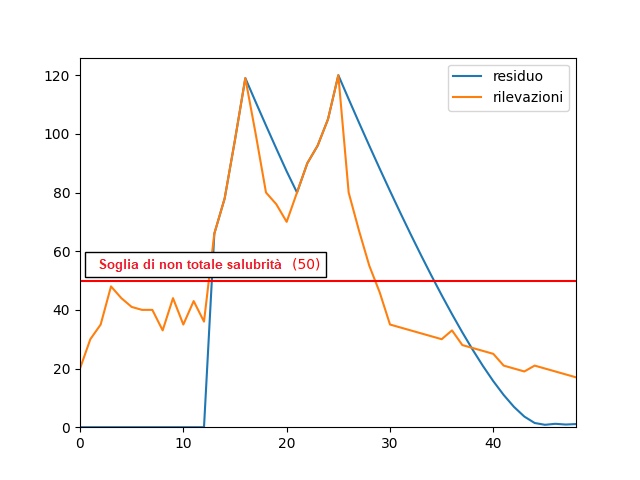
\includegraphics[width=\linewidth]{img/residue.png}
  \caption{L'andamento del residuo con delle possibili rilevazioni.}
  \label{fig:residue}
\end{figure}








\subsection{Generazione del Sub Bass di sottofondo} 
La traccia di sub-bass viene generata tramite un algoritmo implementato nei file sub e wave buffer.
Questa è l'unica traccia che viene effettivamente sintetizzata, e non è basata su note MIDI.
L'unico parametro di cui il processo ha bisogno è l'array di dati relativi alle varie rilevazioni, l'oggetto prodotto è un array di campioni audio stereo.
\subsubsection{Suddivisione dei dati in intervalli}
Il primo passo che questo sottosistema svolge è quello di dividere tutte le rilevazioni in sottointervalli di AQI consecutivi non ottimali.
Per ogni sottointervallo, ne viene indicato l'indice di inizio e quello di fine.
\subsubsection{Generazione delle WaveTable}
In seguito alla suddivisione, per ogni intervallo viene generata una WaveTable.
Per prima cosa viene prelevato il sub-array di dati relativo all'intervallo, in segutio, tramite la classe specificata in wavebuffer.py (listato ~\ref{lst:wavebuffer}), viene creato l'array di campioni wavetable.
Partendo dai dati grezzi, ovvero le sole rilevazioni AQI, il primo passo che la classe svolge è quello di aggiungere all'array una sua copia negativa, in modo da rispettare l'ampiezza massima e minima di un segnale audio.
In seguito vengono aggiunti, tramite interpolazione periodica, tanti punti quanti sono i campioni che la WaveTable deve contenere, nel mio caso, 8192.
Ho scelto l'interpolazione periodica per fare combaciare sempre il primo campione con l'ultimo, rendendo l'onda effettivamente continua.
A seguito dell'interpolazione, ogni campione viene attenuato, ogni valore nella wavetable viene quindi mappato in un numero compreso tra 1 e -1.
Infine, al segnale viene applicato un filtro "Sample n Hold": un circuito che, preso come input un segnale, ne diminuisce la frequenza di campionamento.
L'intervallo di campionamento per il Sample n Hold è stabilito dall'AQI medio, più è alto, più l'onda perde di segnale e risulta invasiva.
\\
\begin{figure}[h]
  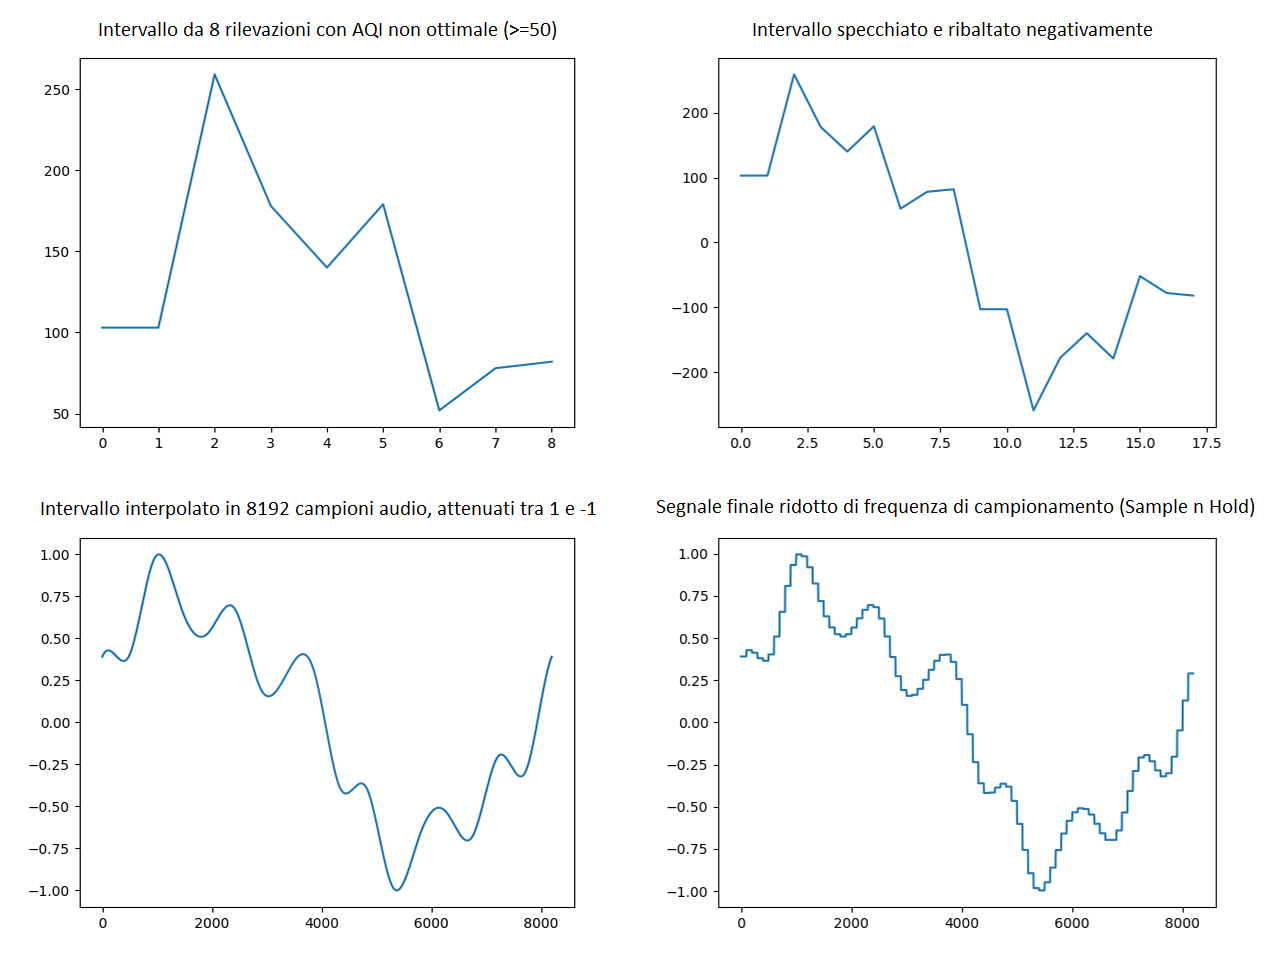
\includegraphics[width=\linewidth]{img/waves.png}
  \caption{Le fasi della generazione di una WaveTable.}
  \label{fig:wave_sub}
\end{figure}

\newpage

\begin{lstlisting}[language=Python,caption={La classe che si occupa della generazione di WaveTable.},label={lst:wavebuffer}]
class WaveBuffer(object):

  def __init__(self, buffer):
      self.buffer = buffer

  # map every value between amp_targer and amp_target * -1
  def amplify(self, amp_target = 1):
      max_item = max(self.buffer)
      amp = amp_target / max_item
      return WaveBuffer([sample * amp for sample in self.buffer])

  # add a copy of the buffer with inverted values
  def mirror_extend(self):
      half_len = len(self.buffer)        
      mirrored = self.buffer + self.buffer
      return WaveBuffer([mirrored[i] if i < half_len else mirrored[i] * -1 for i in range(len(mirrored))])

  # interpolate buffer to given point number (default is 8192)
  def interpolate(self, points = WAVETABLE_SIZE): # 8192 = default wavetable size
      y = self.buffer
      x = np.arange(len(y))
      spl = splrep(x, y, per=True)
      newx = np.linspace(0, len(y)-1, points)
      return WaveBuffer(splev(newx, spl))

  # apply a sample and hold filter to the buffer
  def quantize(self, samples):
      return WaveBuffer([self.buffer[math.floor(i / samples) * samples] for i in range(len(self.buffer))])

  # return the buffer
  def get_buffer(self):
      return self.buffer
\end{lstlisting}



\subsubsection{Preparazione dei modificatori di volume: LFO, Enveloper}
Prima di passare alla sintesi vera e propria, il sottosistema definisce gli elementi necessari per l'andamento dinamico del volume.
Gli elementi sono l'LFO e l'Enveloper.
In questa sonificazione, l'LFO appare come una funzione sinusoidale periodica che oscilla tra 0.5 e 1.5, i valori che andranno a moltiplicarsi al volume.
L'LFO viene restituito sotto forma di lambda dalla seguente funzione (listato ~\ref{lst:lfo}).

\begin{lstlisting}[language=Python,caption={Generazione dell'LFO.},label={lst:lfo}]
def compute_LFO(min, max, samp_period): 
    # samp_period = distanza in campioni tra i picchi della funzione
    freq = 1 / (samp_period / SAMPLE_RATE)
    period = SAMPLE_RATE / freq
    half = (max - min) / 2
    return lambda x: math.sin(2.0 * math.pi * (x) / period) * half + half + min
\end{lstlisting}
L'enveloper appare come una semplice funzione che, preso come parametro un array di campioni, ne attenua l'inizio e la fine (listato ~\ref{lst:enveloper}).

\begin{lstlisting}[language=Python,caption={La funzione Enveloper.},label={lst:enveloper}]
def envelope_buffer(buffer):

  nsamples    = len(buffer)
  attack_s    = nsamples * 0.1
  decay_s     = nsamples * 0.1

  for i in range(nsamples):
      if i < attack_s:
          buffer[i] *= map_value(i, 0, attack_s, 0, 1)
      if i > nsamples - decay_s:
          buffer[i] *= map_value(i, nsamples - decay_s, nsamples, 1, 0)

  return buffer
\end{lstlisting}

\subsubsection{Sintesi}
Si può passare alla funzione di sintesi vera e propria (listato ~\ref{lst:audio_buffer}).
La prima cosa svolta dalla funzione è definire le metriche della traccia, quali il tempo, il numero di note per intervallo, la frequenza di campionamento e la tonalità che si vuole rappresentare.
Per ogni intervallo viene generato un buffer audio, questi verranno poi concatenati in un unico array.
Ogni intervallo è composto da più rilevazioni, ognuna delle quali verrà sonificata con quattro note; il volume e la durata di ogni nota è definita dalla gravità dell'AQI della rilevazione.
I campioni inseriti nel buffer vengono presi dalla WaveTable relativa all'intervallo.
Il valore di ogni campione viene moltiplicato per il volume e per il relativo valore della funzione LFO.
Al fine nascondere le discontinuità delle onde nelle note suonate, il buffer di ognuna di queste viene processato dalla fuzione Enveloper, che attenua i primi e gli ultimi campioni.


\begin{lstlisting}[language=Python,caption={Generazione del buffer audio.},label={lst:audio_buffer}]
def get_wav(data, intervals, wavetables, B):

  B_PER_SEC   = BPM / 60                  # beats per second
  SECONDS     = B / B_PER_SEC             # total track seconds
  SAMPLES     = SECONDS * SAMPLE_RATE     # total track samples

  NOTE_FREQ   = 65.41                                         # C2
  NOTES_PER_B = 4                                             # notes per beat
  STEP        = (NOTE_FREQ * WAVETABLE_SIZE) / SAMPLE_RATE    # wavetable step
  SAMPS_PER_N = int(SAMPLE_RATE / B_PER_SEC / NOTES_PER_B)    # samples per note

  LFO         = compute_LFO(0.5, 1.5, SAMPLE_RATE // B_PER_SEC)
  buff        = np.zeros(int(SAMPLES))
  lfo_ptr     = 0

  # iterate over intervals
  for interval_idx in range(len(intervals)):

      interval    = intervals[interval_idx]
      start, end  = interval[0], interval[1]
      wavetable   = wavetables[interval_idx]

      # iterate over measurements in interval
      for data_idx in range(start, end):

          aqi = data[data_idx]
          vol = map_value(aqi, MIN_THRESH, MAX_THRESH, 0, 0.05)
          dur = map_value_int(aqi, MIN_THRESH, MAX_THRESH, SAMPS_PER_N // 4, SAMPS_PER_N)

          # each measurements has 4 consecutive notes
          for note_idx in range(NOTES_PER_B):

              note_start  = math.floor((data_idx + (note_idx / NOTES_PER_B)) * (SAMPLE_RATE / B_PER_SEC))
              note_buff   = np.array([wavetable[math.floor(i * STEP) % WAVETABLE_SIZE] * vol * LFO(i + lfo_ptr) for i in range(dur)])
              env_buffer  = envelope_buffer(note_buff)
              lfo_ptr     += dur
              buff[note_start:note_start + dur] += env_buffer

  return buff
\end{lstlisting}

\section{Merging delle tracce}
Una volta pronti gli array di tutte le traccie audio, questi vengono uniti in un'unica lista, che viene salvata su un file .wav.
Per evitare errori, ad ogni array viene aggiunto un padding di campioni nulli per rendere tutti i buffer della stessa lunghezza (listato ~\ref{lst:padding}).

\begin{lstlisting}[language=Python,caption={Aggiunta del padding.},label={lst:padding}]
def merge_and_save(*tracks):
  # find max number of samples of track with max num of samples
  # then add padding and merge by sum
  maxlen  = max([len(track[1]) for track in tracks])
  padded  = [np.pad(track, ((0,0), (0, maxlen - len(track[0]))), 'constant', constant_values=0) for track in tracks]
  final   = np.sum(padded, axis=0)
\end{lstlisting}



\section{Generazione del video}
L'animazione è composta da tanti frame quante le rilevazioni di AQI presenti nel dataset.
Per ognuno di questi frame viene aggiunta una legenda che assegna ad ogni colore un fattore di rischio.
Le rilevazioni sono rappresentati con delle barre, mentre il residuo da una linea continua.
In Figura \ref{fig:video} viene mostrato un possibile frame della simulazione.
\begin{figure}[h]
  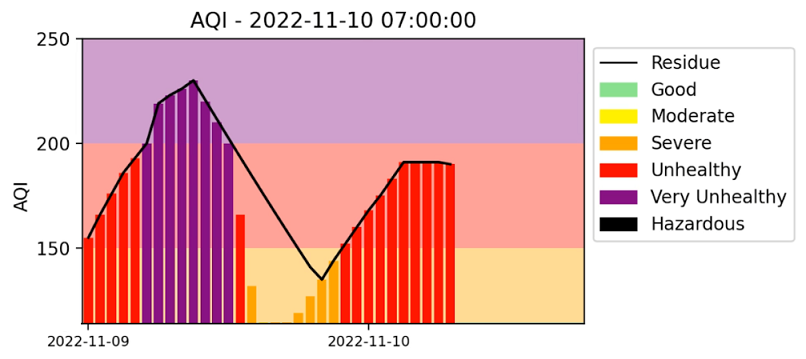
\includegraphics[width=\linewidth]{img/video.PNG}
  \label{fig:video}
\end{figure}



\section{Testing}
\subsection{Test su dispositivi}
In seguito allo sviluppo, l'applicativo è stato testato su diversi browser installati su diversi dispositivi.
I browser utilizzati sono stati Chrome, Opera, Safari e Brave, utilizzati su dispositivi Android, iOS, Windows e Linux.
Sono stati effettuati test da personal computer, smartphone e tablet di diverse risoluzioni.
In Figura \ref{fig:mobile} viene mostrata la schermata responsiva mobile su IPhone SE.

\begin{figure}[h]
  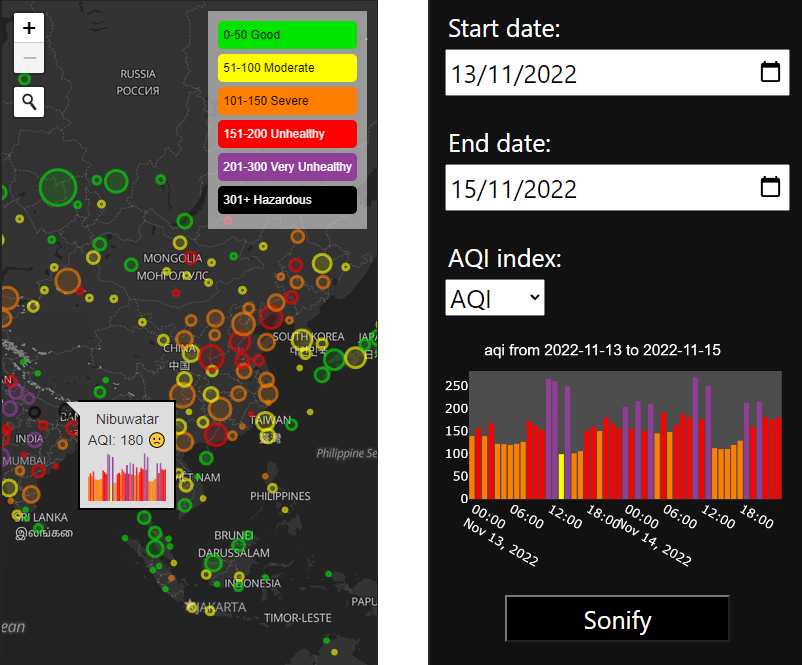
\includegraphics[width=\linewidth]{img/mobile.png}
  \label{fig:mobile}
  \caption{La schermata principale su IPhone SE.}
\end{figure}

\subsubsection{Problemi riscontrati}
Durante il test su dispositivi iOS, ho riscontrato dei problemi riguardanti la riproduzione del video.
In particolare, nonostante questo fosse visualizzato correttamente, era privo di suono.
Il problema è stato individuato visualizzando file di diversi formati su browser, questo riguardava l'incopatibilità della codifica video da parte del dispositivo.
Per risolvere questo problema, ho deciso di non utilizzare più la libreria moviepy, e di richiamare direttamente ffmpeg per unire audio e animazione.
Un secondo problema riscontrato riguardava sempre l'assenza dell'audio sul browser Brave. Il problema è stato risolto disabilitando la funzione di auto riproduzione del video. 

\subsection{Questionario SUS}
SUS (System Usability Scale) è un questionario di valutazione, sviluppato da John Brooke nel 1986 \cite{sussurvey}.
Grazie alla sua semplicità ed efficacia, è stato nominato standard internazionale per la valutazione dell'usabilità di sistemi informatici.
La formula SUS è composta da 10 domande, i cui punteggi vanno da 1 a 5; le domande riguardano principalmente la facilità d'uso, la comprensione e la soddisfazione dell'utente.

\subsubsection{Domande del questionario}
Il questionario alterna domande positive e negative, per differenziare il feedback dell'utente.
Di seguito, vengono riportate le domande del questionario, tradotte in italiano.
\begin{itemize}
  \item Penso che mi piacerebbe utilizzare questo sistema più frequentemente;
  \item Ho trovato il sistema troppo complesso senza che ce ne fosse il bisogno;
  \item Ho trovato il sistema semplice da utilizzare;
  \item Sento il bisogno di assistenza nell'utilizzo del sistema;
  \item Ritengo che le varie funzioni del sistema siano state ben integrate;
  \item Ho riscontrato troppe inconsistenze nel sistema;
  \item Ritengo che gran parte delle persone siano in grado di utilizzare il sistema;
  \item Ho trovato il sistema macchinoso da utilizzare;
  \item Ho provato confidenza nell'utilizzo del sistema;
  \item Dovrei imparare troppe cose prima di utilizzare il sistema al meglio.
\end{itemize}

\subsubsection{Calcolo del punteggio}
I passi per il calcolo del punteggio SUS sono i seguenti:
\begin{enumerate}
  \item Si sommano i punteggi delle domande dispari, e gli si sottrae 5;
  \item Si sommano i punteggi delle domande pari, e gli si sottrae 25;
  \item La somma di questi due numeri ottenuti viene moltiplicata per 2.5, in modo da ottenere un numero compreso tra 0 e 100.
\end{enumerate}
Per avere un riscontro immediato sul punteggio ottenuto, è possibile consultare Figura \ref{fig:sus}:

\begin{figure}[h]
  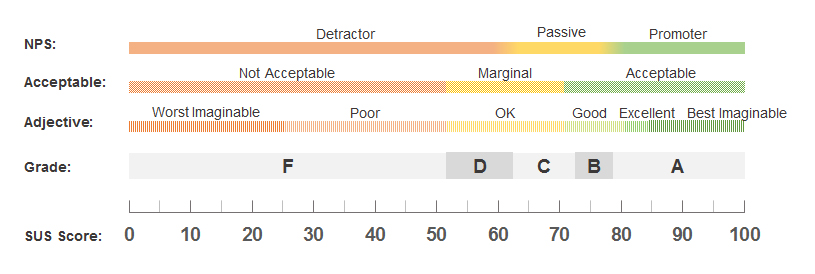
\includegraphics[width=\linewidth]{img/sus.jpg}
  \caption{Tabella con i punteggi SUS \cite{sus}.}
  \label{fig:sus}
\end{figure}

\subsubsection{Punteggio totalizzato}
Dopo avere utilizzato l'applicativo per un periodo di tempo, il questionario è stato compilato da 12 utenti.
Questi sono 6 compagni di corso, 4 studenti di un altro corso di studio e 2 conoscenti non particolarmente pratici di sistemi informatici.
L'età media degli utenti è di 22 anni, 10 sono maschi e 2 femmine.
Il punteggio ottenuto è stato di 89.5, somalente un campione ha riportato un punteggio inferiore a 80.
La fase di open beta ha permesso di raccogliere feedback e suggerimenti da parte degli utenti, sottolineando eventiali aspetti da migliorare.
I risultati ottenuti sono riportati in Figura \ref{fig:result}, le colonne rappresentano le risposte medie alle domande, i cui indici sono gli stessi riportati precedentemente; le domande positive sono colorate di blu, mentre quelle negative di rosso.

\begin{figure}[h]
  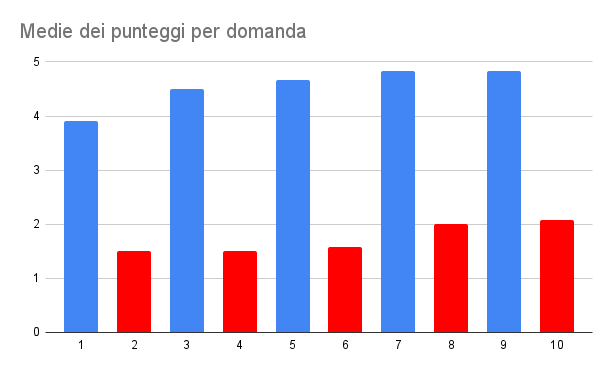
\includegraphics[width=\linewidth]{img/media.png}
  \caption{I risultati del sondaggio.}
  \label{fig:result}
\end{figure}

	

	%%%%%%%%%%%%%%%%%%%%%%%%%
	% inizio parte finale del documento
	%
	% eventuali appendici, bibliografia obbligatoria,
	% eventuale lista delle tabelle e delle figure (nel caso decommentare 
	% la riga con i comandi \listoffigures e \listoftables)
	%%%%%%%%%%%%%%%%%%%%%%%%%
	
    %%%%%%%%%%%%%%%%%%%%%%%%%%%%%%%%%%%%%%%%%non numera l'ultima pagina sinistra
\clearpage{\pagestyle{empty}\cleardoublepage}
%%%%%%%%%%%%%%%%%%%%%%%%%%%%%%%%%%%%%%%%%per fare le conclusioni
\chapter*{Conclusioni}
%%%%%%%%%%%%%%%%%%%%%%%%%%%%%%%%%%%%%%%%%imposta l'intestazione di pagina
\rhead[\fancyplain{}{\bfseries
CONCLUSIONI}]{\fancyplain{}{\bfseries\thepage}}
\lhead[\fancyplain{}{\bfseries\thepage}]{\fancyplain{}{\bfseries
CONCLUSIONI}}
%%%%%%%%%%%%%%%%%%%%%%%%%%%%%%%%%%%%%%%%%aggiunge la voce Conclusioni
                                        %   nell'indice
Questo progetto si è posto l'obbiettivo di creare un'applicazione web interattiva che permetta di visualizzare e sonificare i dati relativi all'inquinamento atmosferico.
Lo sviluppo è stato preceduto da una fase di analisi, definizione dei requisiti e progettazione, che ha portato alla scelta delle tecnologie e strategie da utilizzare.
L'adozione di questo approccio ha permesso uno sviluppo del sistema gradevole e divertente, e ha permesso di acquisire nuove competenze e conoscenze.
Tramite i test effettuatii, è stato possibile verificare che l'applicazione soddisfa i requisiti richiesti, e che l'interfaccia è intuitiva e facile da utilizzare.
La fase di open beta ha permesso di raccogliere feedback e suggerimenti da parte degli utenti, sottolineando eventiali aspetti da migliorare.
In generale, i risultati ottenuti sono soddisfacenti.

\subsubsection{Sviluppi futuri}
Siccome l'applicazione è stata sviluppata in un periodo di tempo relativamente breve, è possibile che alcuni aspetti non siano stati adeguatamente implementati.
Per un eventuale sviluppo futuro, è possibile che si vogliano aggiungere nuove funzionalità riguardanti la pagina web interattiva; in particolare, l'applicativo manca di un sistema di login ed autenticazione,
necessario per l'aggiunta di una funzione di storico delle sonificazioni svolte, arricchita da statistiche sull'utilizzo dell sistema e sui dati visualizzati.

    \clearpage{\pagestyle{empty}\cleardoublepage}


\rhead[\fancyplain{}{\bfseries BIBLIOGRAFIA}]{\fancyplain{}{\bfseries\thepage}}
\lhead[\fancyplain{}{\bfseries\thepage}]{\fancyplain{}{\bfseries BIBLIOGRAFIA}}
%%%%%%%%%%%%%%%%%%%%%%%%%%%%%%%%%%%%%%%%% aggiunge l'intestazione di pagina

\addcontentsline{toc}{chapter}{Bibliografia}
%%%%%%%%%%%%%%%%%%%%%%%%%%%%%%%%%%%%%%%%% aggiunge la voce Bibliografia nell'indice





\bibliography{backMatter/biblio}{}
\bibliographystyle{plain}


    \rhead[\fancyplain{}{\bfseries \leftmark}]{\fancyplain{}{\bfseries
\thepage}}
%%%%%%%%%%%%%%%%%%%%%%%%%%%%%%%%%%%%%%%%%aggiunge la voce Bibliografia
                                        %   nell'indice
\addcontentsline{toc}{chapter}{Ringraziamenti}

%%%%%%%%%%%%%%%%%%%%%%%%%%%%%%%%%%%%%%%%%non numera l'ultima pagina sinistra
\clearpage{\pagestyle{empty}\cleardoublepage}
\chapter*{Ringraziamenti}
\thispagestyle{empty}
Qui possiamo ringraziare il mondo intero!!!!!!!!!!\\
Ovviamente solo se uno vuole, non \`e obbligatorio.
	
		
	%\input{./Appendice/appendice.tex}
	%\clearpage{\pagestyle{empty}\cleardoublepage}


\rhead[\fancyplain{}{\bfseries BIBLIOGRAFIA}]{\fancyplain{}{\bfseries\thepage}}
\lhead[\fancyplain{}{\bfseries\thepage}]{\fancyplain{}{\bfseries BIBLIOGRAFIA}}
%%%%%%%%%%%%%%%%%%%%%%%%%%%%%%%%%%%%%%%%% aggiunge l'intestazione di pagina

\addcontentsline{toc}{chapter}{Bibliografia}
%%%%%%%%%%%%%%%%%%%%%%%%%%%%%%%%%%%%%%%%% aggiunge la voce Bibliografia nell'indice





\bibliography{backMatter/biblio}{}
\bibliographystyle{plain}


	
	\nocite{*}

	%\cleardoublepage
	%\addcontentsline{toc}{chapter}{Bibliografia}


	
	%\listoffigures
	%\listoftables


\end{document}
